\documentclass[11pt,a4paper,twoside,ngerman]{article}

\usepackage{thesisPreamble}
%______________________________________________________________________

\begin{document}

\pagestyle{empty} % Vorerst keine Seitenzahlen
\pagenumbering{alph} % Unsichtbare alphabetische Nummerierung
\selectlanguage{ngerman}

\begin{center}
\textsc{Ludwig-Maximilians-Universität München}\\
Department "`Institut für Informatik"'\\
Lehr- und Forschungseinheit Medieninformatik\\
Prof. Dr. Heinrich Hußmann

\vspace{5cm}
{\large\textbf{Bachelorarbeit}}\vspace{.5cm}

{\LARGE Implementierung und Evaluierung einer\\virtuellen Lernplattform}
\vspace{1cm}

{\large Felix Hamann}\\
geboren am 21. September 1989

\end{center}
\vfill

\begin{tabular}{ll}
Bearbeitungszeitraum: & 16. April 2018 bis 3. September 2018\\
Betreuer: & Mohamed Khamis\\
& Dr. Steffen Jost\\
Verantw. Hochschullehrer: & Prof. Hußmann
\end{tabular}

%______________________________________________________________________

\clearpage
\section*{Zusammenfassung}

Das \textit{Virtual Learning Environment} (\textit{VLE}, Verwaltungs-System für Bildungseinrichtungen) in Form der Webseite \textit{UniWorX}, das an der Ludwig-Maximilian-Universität in München eingesetzt wird, soll durch \textit{Uni2work} ersetzt werden. In dieser Arbeit wird der Entwicklungsprozess von \textit{Uni2work} beschrieben und erste Evaluationsergebnisse dieses neuen Systems präsentiert. Es wird außerdem auf \textit{UniWorX} und alternative VLEs eingegangen.

Die Serverseite von Uni2work wurde in Haskell von Dr. Steffen Jost und Gregor Kleen mit Hilfe des \textit{Yesod Web Frameworks} geschrieben. Die Clientseite und jegliche damit verbundene \textit{User Interface}- und \textit{User Experience}-Arbeit wurde vom Autor durchgeführt und in Form von HTML-Templates umgesetzt. 

Für eine erste Evaluierung des Systems wurde der \textit{System Usability Scale} (\textit{SUS}), mit dem sich die Bedienbarkeit (\textit{Usability}) von Systemen bemessen und vergleichen lässt, in einer Umfrage eingesetzt. Die resultierenden SUS-Werte für das aktuelle System \textit{UniWorX} und dem geplanten Ersatz \textit{Uni2work} sprechen lediglich für eine marginal bessere Bedienbarkeit von \textit{UniWorX}. Die qualitative Auswertung der in der Umfrage gestellten offenen Fragen deutet hingegen auf eine bessere Bedienbarkeit des neuen Systems und eine deutlich bessere Bedienbarkeit des Systems auf mobilen Geräten hin.

Außerdem werden Folgeschritte für die Zukunft vorgestellt die sich bei der Auswertung der Umfrage als nötig oder wünschenswert erwiesen haben.

\selectlanguage{english}
\section*{Abstract}

Short abstract of the work, maximum of 250 words.

\selectlanguage{ngerman}
\clearpage
\section*{Aufgabenstellung}

Kopie der Original-Aufgabenstellung

\vfill % Sorgt dafür, dass das Folgende an das Seitenende rutscht

\noindent Ich erkläre hiermit, dass ich die vorliegende Arbeit
selbstständig angefertigt, alle Zitate als solche kenntlich gemacht
sowie alle benutzten Quellen und Hilfsmittel angegeben habe.

\bigskip\noindent München, \today

\vspace{4ex}\noindent\makebox[7cm]{\dotfill}

%______________________________________________________________________

\cleardoublepage
\pagestyle{fancy}
\pagenumbering{roman} % R�mische Seitenzahlen
\setcounter{page}{1}

% Inhaltsverzeichnis erzeugen
\tableofcontents

%Abbildungsverzeichnis erzeugen - normalerweise nicht nötig
%\cleardoublepage
%\listoffigures
%______________________________________________________________________

\clearpage

% Arabische Seitenzahlen
\pagenumbering{arabic}
\setcounter{page}{1}
% Geändertes Format für Seitenränder, arabische Seitenzahlen
\fancyhead[LE,RO]{\rightmark}
\fancyhead[LO,RE]{\leftmark}
\fancyfoot[LE,RO]{\thepage}

\section{Einleitung} \label{sec:introduction}
Die Digitalisierung schreitet in immer größer werdenden Schritten voran. Das Internet übernimmt im Bereich der Bildung eine immer größere Rolle. Interessierte können beinahe alles, aus den unterschiedlichsten Bereichen des Internets erlernen. Eine Meldung die derzeit auf diversen News-Seiten kursiert berichtet zum Beispiel von Cara Brookins, einer Frau aus den USA, die innerhalb weniger Jahre und ausschießlich mit Hilfe von Youtube-Videos ein eigenes zweistöckiges Haus baute \cite{web:nyyoutubehouse}. Neben der weithin bekannten Videoplattform \textit{Youtube} haben sich auch viele dedizierte Lern-Plattformen etabliert. Bekannte Vertreter solcher Plattformen sind \textit{Khan-Academy} \footnote{\url{https://khanacademy.org/}}, \textit{Udemy} \footnote{\url{https://udemy.com/}}, \textit{Udacity} \footnote{\url{https://udacity.com/}} und \textit{Lynda} \footnote{\url{https://lynda.com/}}. Diese Seiten stellen großteils \textit{Virtual Learning Environments} dar, in welchen Lernende Zugriff auf Lehrmaterialien, Tests, Fortschrittsprotokolle und Anderes erhalten.

\subsection{Virtual Learning Environment (VLE)} \label{sec:intro-vle}

\begin{figure}[h]
    \centering
    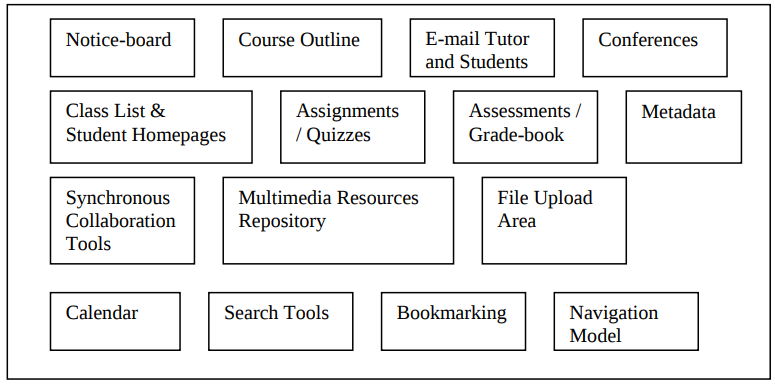
\includegraphics[width=13cm]{images/protovle.png}
    \caption{Schema eines prototypischen VLE \cite{jtap-vle}}
    \label{fig:prototypical_vle}
\end{figure}

\noindent
Ein Virtual Learning Environment ist ein System in Form einer Webseite im Intra- oder Internet das Lernenden und Lehrenden das Lernen und Lehren erleichtern soll.

Die positiven Kernaspekte einer VLE wurden bereits 1997 im sogenannten \textit{Dearing Report} zur "`Higher Education in the learning society"' herausgearbeitet \cite{dearing1997}.
Diese wurden von Sandy Britain und Oleg Liber in ihrer Arbeit zur Evaluierung von VLEs 1999 zusammengefasst \cite{jtap-vle}. Hier eine Auflistung der wichtigsten Aspekte:

\begin{itemize}
    \item Flexibilität in Bezug auf Zeit und Raum
    \item Bewältigung einer wachsenden Anzahl von Studenten
    \item Teilen und Wiederverwenden von Ressourcen
    \item Kollaboratives Zusammenarbeiten von Studenten und Tutoren
    \item Reduzierung der administrativen Last
\end{itemize}

\noindent
In ihrer Arbeit halten sie die wichtigsten Funktionalitäten einer VLE in einem Schema \autoref{fig:prototypical_vle} fest, an dem sich seit nunmehr 20 Jahren nichts grundlegendes geändert hat. Alle in dieser Abbildung dargestellten Funktionalitäten finden auch heutzutage in VLEs Verwendung, wobei ein System nicht alle davon bieten muss um als VLE bezeichnet werden zu können. \cite{jtap-vle}

Die \textit{University and Colleges Information Systems Association} (UCISA) \footnote{\url{https://www.ucisa.ac.uk/}} veröffentlichte 2016 zum neunten Mal eine Studie zum Thema \textit{Technology Enhanced Learning} (TEL). TEL bezeichnte jede Online-Einrichtung und jedes technische System welches Lernen und Lehren direkt unterstützt oder ermöglicht. Das Ziel dieser Umfrage ist es einen Überblick über die in Großbritannien im Einsatz befindlichen VLEs und deren Entwicklung zu bekommen. Seit spätestens 2012 stehen \textit{Moodle} und \textit{Blackboard Learn} an erster Stelle bei der Häufigkeit der eingesetzten VLEs. Von Jahr zu Jahr zunehmendes Interesse ist der Verfügbarkeit und angemessenen Bedienbarkeit der universitären Seiten auf mobilen Geräten mit kleinen Bildschirmen gewidmet \cite{ucisa-tel16}\cite{web:ucisatel}.

\subsection{Motivation}
Auch an Universitäten kommen VLEs zum Einsatz. An der Ludwig-Maximilians-Universität in München sind es sogar mehrere. Diese somit zur Verfügung gestellten Plattformen und Werkzeuge sollen grundsätzlich dazu dienen die Produktivität und Effizienz der Mitarbeiter der Universität und der Studenten zu erhöhen. Viele der Webseiten die diese Werkzeuge zugänglich machen wurden jedoch vor teilweise mehr als 10 Jahren entwickelt und blieben von dem rasanten Wandel des Internets \footnote{Web 2.0, Web 3.0, Web 4.0, \ldots} in dieser Zeit größtenteils unberührt. Sie sind somit einerseits nicht mehr auf dem aktuellen Stand der Technik, andererseits haben sich auch Design- und Bedienbarkeitsansprüche in der Zwischenzeit wesentlich gewandelt.

Weil sich an der LMU mehrere VLEs zu einem Gesamtsystem vernetzen, verlangt der studentische Alltag das regelmäßige Wechseln zwischen Vorlesungswebseiten und den Übungs- und Klausurenplattformen. Manche Kurse, Vorlesungen und Seminare setzen darüber hinaus weitere spezifische Tools ein um den Unterricht zu gestalten.

Für LMU-Studenten der Medieninformatik stellt das System \textit{UniWorX} das wohl Zentralste dieser Werkzeuge dar. Auch UniWorX entspricht nicht mehr dem aktuellen Stand der Technik und soll durch einen modernen Nachfolger ersetzt werden. Dieser soll über einen größeren Funktionsumfang verfügen und andere VLEs, die derzeit parallel zu UniWorX betrieben werden, überflüssig machen. Den Studenten soll insbesondere der Zugang auf mobilen Geräten erleichtert werden und die Usability auf aktuelle Standards angehoben werden.

\subsection{Herangehensweise}
Das bestehende VLE UniWorX, das seit 2009 an der LMU im Einsatz ist und seitdem mehrmals überarbeitet wurde \cite{web:pstifiuniworx}\cite{web:uniworxchangelog} soll im Rahmen dieser Arbeit in Form des neuen VLEs \textit{Uni2work} unter Einbeziehung bewährter Lösungsansätze auf den aktuellen Stand der Technik gebracht werden. Das neue System soll insgesamt besser in die studentischen Prozesse an der LMU integriert werden.

Nach der ersten Entwicklungsiteration wurde eine Studie durchgeführt deren Teilnehmer einen Fragebogen ausfüllen mussten in dem unter anderem der \textit{System Usability Scale} (SUS) zum Einsatz kam. Mit Hilfe des SUS lässt sich die Usability von Systemen über Disziplinen hinweg mit einer Messzahl versehen und vergleichen. Näher auf SUS, die generelle angewandte Methode, weitere gestellte Fragen und deren Auswertung wird in \autoref{sec:userstudies} eingegangen.

ELABORATE?

\clearpage
\section{Status Quo -- Das System \textit{UniWorX}} \label{sec:uniworx}
Die LMU setzt seit 2009 für ihre Informatik-nahen Studiengänge \footnote{Hauptsächlich: Informatik, Bioinformatik, Medieninformatik} die VLE \emph{UniWorX} ein. Jeder berechtigte Mitarbeiter und Student der LMU verfügt dort über ein Benutzerkonto. Das System dient Studenten als zentraler Ort für die Lösungsabgabe und das Herunterladen von Übungsblättern und die Anmeldung zu Kursen und Klausuren. Das Herunterladen von Kursmaterialien wie Präsentationsfolien geschieht jedoch zum größten Teil über die entsprechenden, von den Dozenten und Fakultäten verwalteten Seiten der entsprechenden Kurse -- im Wesentlichen isoliert von UniWorX.

Mit UniWorX wird sowohl den Dozenten und Tutoren als auch den Studenten die Arbeit dahingehend erleichtert, als dass es für manche Aktivitäten des studentischen Alltags eine zentrale Anlaufstelle bereitstellt. Diese Aktivitäten, die verschiedenen Rollen im System und die Architektur des Systems UniWorX sollen in den folgenden Unterabschnitten genauer erläutert werden.

\begin{figure}[h]
    \centering
    
\includegraphics[width=.9\textwidth]{images/uniworx_promo.png}
    \caption{UniWorX 2: Veranstaltungsseite \textit{Programmierung und Modellierung}}
    \label{fig:uniworx_promo}
\end{figure}

\subsection{Entwicklung} \label{sec:uniworx_development}
UniWorX ist eine öffentliche Webplattform und wird auf den Servern der LMU betrieben. Die Webseite ist somit weltweit über die URL \url{https://uniworx.ifi.lmu.de} erreichbar.

\subsubsection{UniWorX 1}
Die erste Version von UniWorX wurde bis September 2010 am Lehrstuhl für Programmierung \& Softwaretechnik der LMU entwickelt. Während es im Einsatz war wurden kontinuierlich Verbesserungen in Form von kleinen Aktualisierungen hinzugefügt die hauptsächlich dem Beheben von Bugs dienten.

Die letzte Aktualisierung (UniWorX 1.6.19) wurde am 17. September 2010 veröffentlicht und etwa ein Jahr später am 25. September 2011 durch UniWorX 2 abgelöst. Das bis dahin bestehende UniWorX wurde den damaligen Studenten als Archiv zur Verfügung gestellt und ist heute nicht mehr öffentlich zugänglich. \cite{web:pstifiuniworx}

\subsubsection{UniWorX 2}
UniWorX 2 wurde in der Programmiersprache PERL \footnote{Perl: Write once – never understand again.} neu geschrieben.
Nach einer zweiwöchigen Testphase mit ausgewählten Testern ging das System zum Wintersemester 2011/2012 in den Produktivbetrieb und löste das bis dahin verwendete System UniWorX 1 als \textit{Public Beta} \footnote{Phase eines Programms in der es \textit{ohne vollständige Garantie auf Fehlerfreiheit} von der (eingeschränkten) Öffentlichkeit benutzt werden kannn} ab \cite{web:uniworxchangelog}. Eine Umfrage begleitete das Ende der Beta Phase, um die Benutzer nach der Usability zu fragen und Feedback einzuholen. Auf diese Umfrage, ihre Ergebnisse und somit wertvolle Informationen für einen potenziellen Nachfolger von UniWorX 2 wird im folgenden \autoref{sec:uniworx_survey} genauer eingegangen. \autoref{fig:uniworx_promo} zeigt eine Vorlesungsseite im heute eingesetzten UniWorX 2.

\subsection{UniWorX 2-Studie} \label{sec:uniworx_survey}
Bevor UniWorX 2 zum Sommersemester 2012 seine Beta-Phase beendete wurde eine Umfrage unter den Benutzern durchgeführt an welcher 265 Personen teilnahmen. Damit sollte Feedback gesammelt werden um jegliche verbleibende Bugs und womöglich gravierende Fehler für den normalen Betrieb zu begleichen. Unter den Teilnehmern der Umfrage befanden sich 13 Mitarbeiter des beteiligten Instituts. 51\% der Teilnehmer studierten Medieninformatik.
Die Kernthemen der Umfrage waren die allgemeine Usability und bei der Benutzung aufgetretene Probleme, Bedenken und Bugs. \autoref{fig:uniworx_satisfaction} zeigt die deutliche Zufriedenheit der Teilnehmer mit UniWorX.

Ein gravierender Kritikpunkt der sich aus den Umfrageergebnissen ergab waren die fehlenden Veranstaltungen anderer Institute und Fakultäten in UniWorX.

\begin{figure}[h]
    \centering
    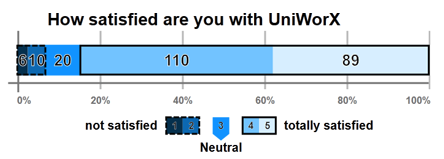
\includegraphics[width=10cm]{images/uniworx_satisfaction.png}
    \caption{Grafik aus den Ergebnissen der 2012 durchgeführten UniWorX 2 Umfrage. Über 80\% der Teilnehmer der Studie waren mit UniWorX zufrieden. \\ Quelle: \url{https://uniworx.ifi.lmu.de/survey/}}
    \label{fig:uniworx_satisfaction}
\end{figure}

\subsection{Benutzerrollen} \label{sec:uniworx_users}
In UniWorX existieren verschiedene Rollen die von den unterschiedlichen Benutzern eingenommen werden können. Es wird grob zwischen \textbf{Administratoren}, \textbf{Dozenten/Assistenten}, \textbf{Tutoren} und \textbf{Studenten} unterschieden.

\begin{itemize}
    \item \textbf{Studenten} \hfill \\ 
    können in UniWorX die Veranstaltungsliste (enthält Kurse, Seminare, Praktika usw.) einsehen und sich zu (offenen) Veranstaltungen anmelden. Entsprechend der Veranstaltung können Studenten nach erfolgreicher Anmeldung Übungsblätter herunterladen und ihre Lösungen anonym hochladen und sich für Klausuren an- oder abmelden. Für Veranstaltungen die einer Bewerbung bedürfen können Studenten ein Motivationsschreiben verfassen und direkt über UniWorX einreichen. Über alle wichtigen Neuigkeiten (Bewerbungsstatus, Abgabe-Deadlines, anstehende Klausuren, etc.) werden von UniWorX automatisiert Emails verschickt die von den Studenten feingranular bestellt und abbestellt werden können.
    \item \textbf{Tutoren} \hfill \\ 
    haben in UniWorX die Aufgabe die eingereichten Arbeiten der Studenten zu korrigieren und die korrigierten Lösungen zur Verfügung zu stellen.
    \item \textbf{Dozenten/Assistenten} \hfill \\
    können Veranstaltungen und (falls angemessen) passende Übungsblätter anlegen sowie (falls angemessen) Klausuren dafür eintragen. Für Veranstaltungen wie Seminare bei denen keine wiederkehrenden Abgaben der Studenten erwartet werden, werden keine Übungsblätter und Klausuren angelegt. Zu den Übungsblättern können außerdem Materialien zur Verfügung gestellt werden die über die Oberfläche hochgeladen werden können.
    Die Abgaben der Studenten zu diesen Übungsblättern kann von den Dozenten und Assistenten eingesehen werden. Jeder Abgabe wird beim Hochladen eine eindeutige und anonyme ID zugewiesen um die Identität der Studenten zu verschleiern und Interessenkonflikte beim Korrigieren zu vermeiden. Aufgabe der Dozenten und Assistenten ist es diese Abgaben auf die für den entsprechenden Kurs registrierten Tutoren zu verteilen, wobei diese (Dozenten und Assistenten) selbst ebenfalls Korrekturen durchführen können sofern sie als Tutor eingetragen sind.

    Für Veranstaltungen bei denen die Studenten zur Anmeldung einen Bewerbungsprozess durchlaufen müssen ist es außerdem Aufgabe der Dozenten und deren Assistenten diese Bewerbungen zu sichten und über deren Tauglichkeit zu entscheiden.
    \item \textbf{Administratoren} \hfill \\
    stehen sämtliche Funtkionen der vorigen Benutzerrollen zur Verfügung. Zusätzlich sind sie berechtigt die komplette Benutzerliste von UniWorX einzusehen und Benutzer manuell hinzuzufügen oder zu entfernen.
\end{itemize}

\noindent
Diese Benutzerrollen haben sich als sinnvoll erachtet und sollen so beibehalten werden.

\subsection{Wartbarkeit} \label{sec:uniworx-maintenance}
Bei einem ganztägigen Ausfall von UniWorX und den verbundenen Reparaturen wurde erkannt, dass es nicht möglich ist UniWorX ohne gravierende Änderungen auf neue Hardware zu migrieren. Dies ist jedoch notwendig um der 2018 in Kraft getretenen Datenschutzgrundverordnung (DSGVO) \footnote{Verordnung der EU für einheitliche, EU-weite Datenschutz-Gesetze} gerecht zu werden. Nötige Sicherheitspatches können auf der veralteten Soft- und Hardware nicht installiert werden. Auch Mechanismen wie Virtualisierung \footnote{Ausführen einer Anwendung in einer klar definierten virtuellen Umgebung um stets die gleichen Bedingungen für die Prozesse zu schaffen} und eine Live-Spiegelung der Datenbank um die Verfügbarkeit und Skalierbarkeit des Systems zu gewährleisten kann nicht problemlos implementiert werden.

Täglich werden von UniWorX über 100 Fehlermeldungen und Warnungen produziert, deren Bedeutung aufgrund fehlender Dokumentation nicht immer eindeutig ist.
Die Fehlersuche gestaltet sich auch wegen des sehr stark gekoppelten Codes \footnote{Code deren Komponenten sehr eng miteinander verbunden sind und somit viele Abhängigkeiten bestehen} oft als schwierig. Es besteht insbesondere keine eindeutige Trennung zwischen den Webseiten-Templates, welche die Struktur der Seite definieren, und der nötigen Logik um diese Templates zu befüllen. 

Nach mehreren Jahren im Einsatz erweist sich UniWorX demnach als nicht mehr ausreichend wartbar und erweiterbar, wodurch neue Anforderungen nicht zeitnah umgesetzt werden können. Wegen des Umfangs der nötigen Änderungen die durchgeführt werden müssten um das System DSGVO-konform zu gestalten, wurde entschieden das System grundsätzlich neu zu implementieren. Als Alternative zu einer kompletten Neuimplementierung von UniWorX bot sich die Integration der UniWorX-Aufgaben in eines der anderen bestehenden VLEs der LMU an. In Frage kommen dafür ein modifiziertes Moodle \footnote{weit verbreitetes und quelloffenes VLE, siehe \autoref{sec:intro-vle}} und ein intern entwickeltes Vorlesungsverzeichnis mit VLE-Charakteristiken names LSF \footnote{Lere -- Studium -- Forschung}. Beide dieser Systeme sind hauptsächlich auf die Bereitstellung von Material ausgelegt und werden besonderen Anforderungen an die Handhabung von Korrekturen in UniWorX nicht gerecht, weshalb beschlossen wurde einen Nachfolger zu entwickeln. Im weiteren Verlauf dieser Arbeit ist die Entstehung und anschließende Evaluation dieses UniWorX-Nachfolgers namens Uni2work dokumentiert.

\clearpage
\section{Implementierung von \textit{Uni2work}} \label{sec:implementation}
Der Name "`Uni2work"' (lies: You-nee[d]-to-work) ist zum Zeitpunkt dieser Arbeit noch nicht von allen Beteiligten anstandslos akzeptiert, soll aber als Arbeitstitel im Verlaufe dieser Arbeit der einfacheren Referenzierung dienen.

\subsection{Arbeitsweise} \label{sec:workflow}
Für die organisierte Zusammenarbeit, Versionierung und Protokollierung des Implementierungsprozesses wurde ein gemeinsames Git-Repository eingesetzt welches auf den Servern der LMU über das hauseigene GitLab verwaltet wird. Über die Web-Oberfläche von GitLab wurden Issues und Bugs in Form von \textit{Tickets} festgehalten die innerhalb des Entwickler-Teams kommentiert und einzelnen Entwicklern zugewiesen werden konnten. Aufgrund der kleinen Teamgröße von drei Personen wurde kein spezielles Vorgehensmodell wie Scrum für die Softwareentwicklung verfolgt. Dr. Steffen Jost und HiWi \footnote{Hilfswissenschaftler} Gregor Kleen trafen sich im zwei-wöchigen Turnus um gemeinsam an der Haskell-Seite der Anwendung zu arbeiten. Mit bedarfsbedingt abnehmender Regelmäßigkeit nahm auch der Autor dieser Arbeit an diesen Treffen teil. Die Roadmap und damit einhergehend die anstehenden Entwicklungsschritte wurden zumeist während dieser Treffen und dem anschließenden Email-Verkehr in Form von GitLab-Tickets definiert. Von den bisher etwa 150 geschriebenen Tickets konnten etwa 100 bereits abgearbeitet werden. Der Umfang dieser Tickets reichte von banalen Änderungen wie der Position eines Links auf einer bestimmten Seite bis zu tiefgreifenden architektonischen Entscheidungen.

Automatisiertes Ausrollen der aktuellsten Änderungen (\textit{Continous Integration}) wird über einen extern gehosteten Jenkins-Server \footnote{\url{https://jenkins.io}} betrieben. Das Git-Repository verfügt zu jedem Zeitpunkt über die zwei Branches \footnote{Git-Terminologie: Entwicklungszweig in der Softwareentwicklung} \lstinline!master! und \lstinline!live!. Änderungen in \lstinline!master! veranlassen dessen Ausrollen auf eine Staging-Umgebung in der Änderungen begutachtet und getestet werden können bevor sie der Allgemeint zugänglich gemacht werden. Änderungen des \lstinline!live!-Branches sind nur über die Gitlab-Oberfläche zugelassen und führen zu einem Ausrollen von \lstinline!live! auf die Produktions-Umgebung, die mit SSL-Verschlüsselung unter \url{https://uni2work.ifi.lmu.de} für die Benutzer erreichbar ist.

\subsection{Architektur} \label{sec:uni2work-architecture}
Für die Umsetzung der Webseite des Systems wurde das \emph{Yesod Web Framework} (kurz \emph{Yesod}) für die Programmiersprache Haskell \footnote{Funktionale Programmiersprache, \url{https://www.haskell.org/}} gewählt. Das Setup der Architektur und Yesods wie auch die Programmierung in Haskell wurde von Dr. Steffen Jost und Gregor Kleen durchgeführt. Das Frontend \footnote{Für den Benutzer sichtbarer und spürbarer Teil einer Webseite} wurde vom Autor dieser Arbeit implementiert.

Der Einsatz von Yesod bedingt einen monolithischen Aufbau, in der alle Komponenten der Anwendung in einem gemeinsamen Projekt vereint sind. Yesod übernimmt Datenbeschaffung, -aufbereitung und -darstellung. Für die Datenspeicherung wird eine \textit{PostgreSQL} Datenbank \footnote{\url{https://www.postgresql.org/}} verwendet.
In dieser Arbeit soll insbesondere auf das Frontend und dessen \textit{User Interface} (UI) und die damit verbundene \textit{User Experience} (UX) eingegangen werden. Das Diagramm in \autoref{fig:uni2work-architecture} stellt diese Architektur mit Fokus auf dem Frontend grafisch dar. Die abgebildeten Relationen sind keineswegs maßstabsgetreu: Verglichen an den Codezeilen nimmt das Frontend weniger als 5\% der Anwendung ein. Auf die Inhalte der einzelnen Elemente des Frontends wie Widgets oder Hamlet wird in den nächsten Unterabschnitten eingegangen.

Bei der Umsetzung des Frontends wurde auf die Bedürfnisse aller Benutzer des Systems eingegangen. Die vollumfängliche Benutzbarkeit der Webseite auf alten und/oder leistungsschwachen Geräten und solchen mit kleinen Bildschirmen wurde von Anfang an bei der Umsetzung berücksichtigt.

\begin{figure}[h]
    \centering
    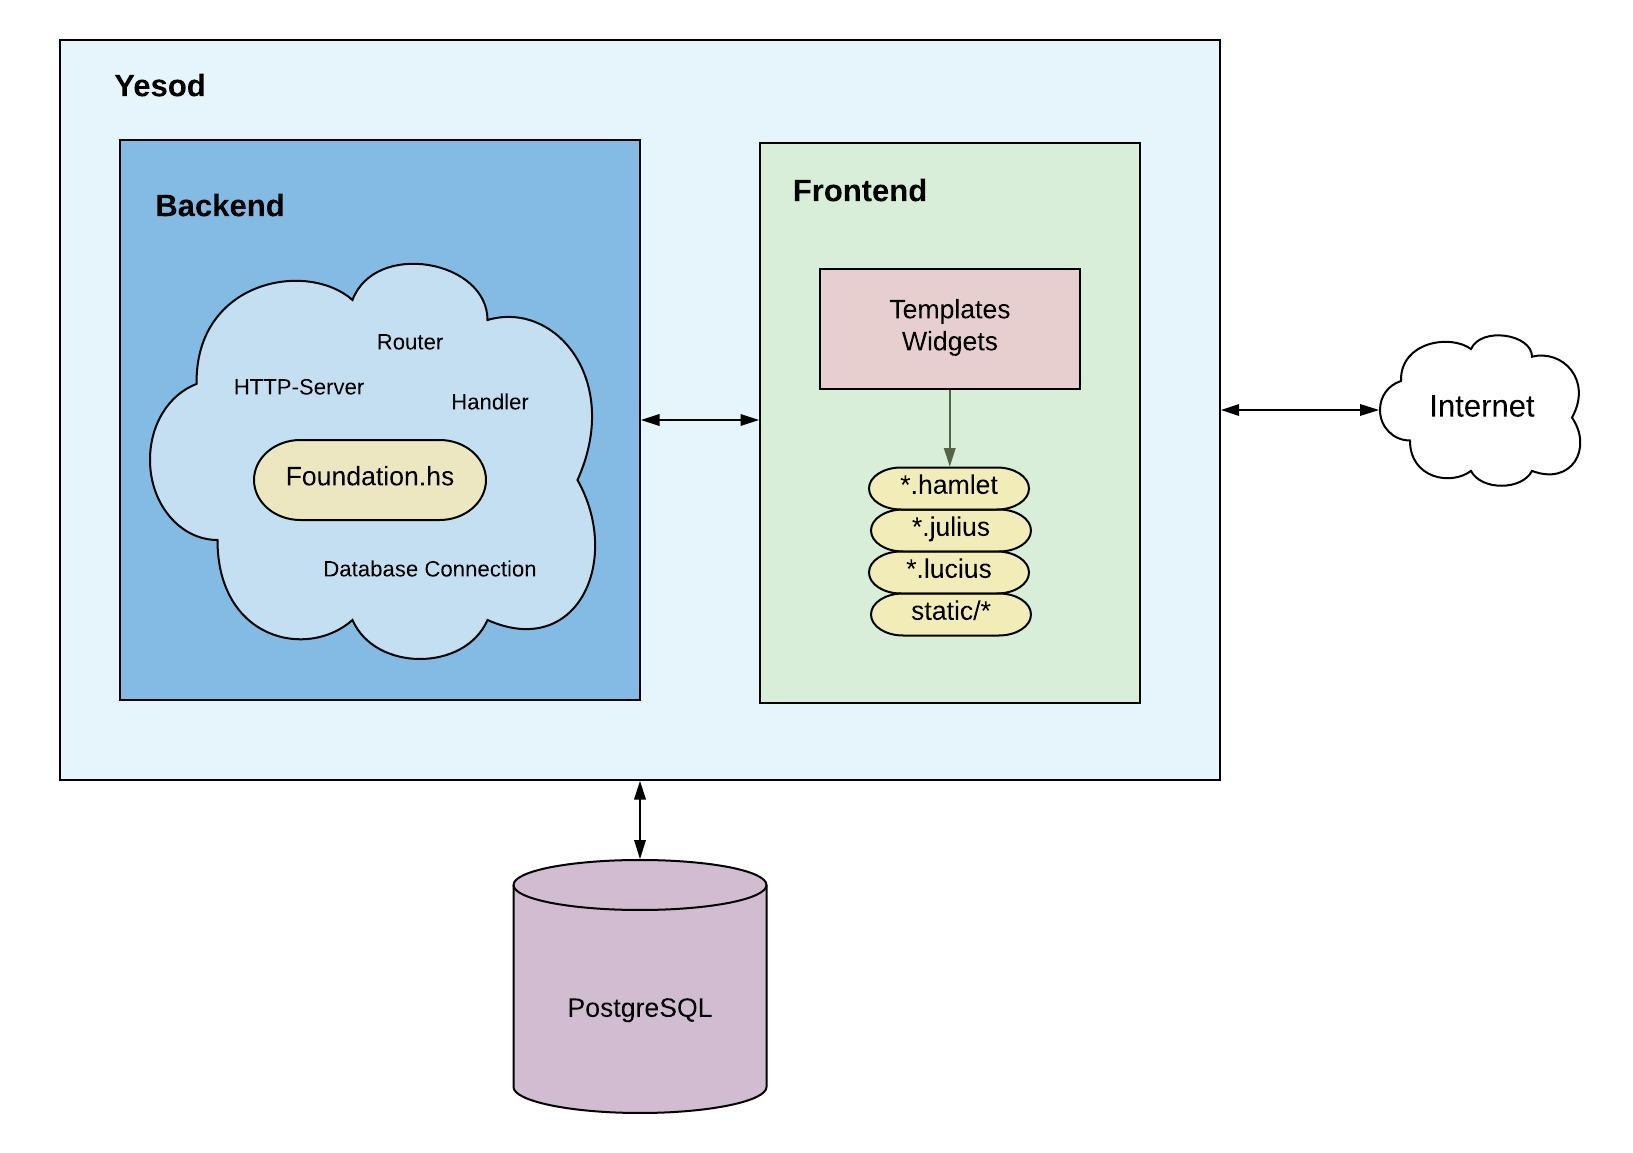
\includegraphics[width=\textwidth]{images/uni2work_architecture.jpeg}
    \caption{Architekturdiagramm von Uni2work}
    \label{fig:uni2work-architecture}
\end{figure}

\subsection{Shakespearean Template Languages} \label{sec:stl}
In dem eingesetzten Haskell-Framework \emph{Yesod} kommt neben Haskell die Sprachfamilie der \emph{Shakespearean Template Languages} zum Einsatz. Diese Sprachfamilie stellt eine Sammlung von vier Sprachen dar, die jeweils sehr eng an HTML, CSS und JavaScript angelehnt sind. Der gemeinsame Vorteil dieser Sprachen ist die Möglichkeit der \textit{Interpolation} von Haskell-Werten beim Kompilieren der Applikation. \cite{web:yesodstl}

\subsubsection{Interpolation} \label{sec:interpolation}
In allen vier Sprachen der Shakespearean Template Languages (\textit{Hamlet, Julius, Cassius, Lucius}) können Haskell-Werte interpoliert werden. Interpolation erlaubt es generische Komponenten zu erstellen, die je nach ihrer Position auf der Webseite mit unterschiedlichem Inhalt erscheinen können.

Da Haskell streng typisiert ist, bedarf es verschiedener Interpolationsmechanismen für die Werte der unterschiedlichen Typen:

\bigskip
\begin{tabular}{l|l}
    String-Interpolation (Zeichenketten einfügen) & \lstinline/#{username}/ \\
    Routen-Interpolation (URLs einfügen) & \lstinline/@{CourseR}/ \\
    Widget-Interpolation (Widget-Code einfügen) & \lstinline/^{widget}/ \\
    Internationalisierungs-Interpolation (Übersetzte Texte einfügen) & \lstinline/_{MessageTerm}/
\end{tabular}

\bigskip
\noindent
Die gezeigten Methoden der Interpolation können in allen vier Sprachen der Shakespearean Template Languages eingesetzt werden, auf die nun genauer eingegangen wird.

\subsubsection{Hamlet, Julius, Cassius \& Lucius}
Yesod bietet mit der Familie der Shakespearean Template Languages vier \textit{eingebettete domänespezifische Sprachen} (EDSL \footnote{Embedded Domain Specific Language}) \cite{web:haskell-edsl}. Diese vier EDSLs vereinen die Sprachen HTML, JavaScript und CSS mit den in \autoref{sec:interpolation} beschriebenen Möglichkeiten der Interpolation und weiteren Funktionen zu \textit{Hamlet} (HTML), \textit{Julius} (JavaScript), \textit{Lucius} (CSS) und \textit{Cassius} (CSS):

\begin{itemize}
    \item \textbf{Hamlet} (HTML) \hfill \\ Eine erweiterte und zugleich vereinfachte Markup-Sprache die zu HTML kompiliert. Statt schließenden HTML-Tags dient in Hamlet Einrückung zum Verschachteln und Abgrenzen von Elementen. \autoref{lst:hamlet-dt} ist ein Beispiel für eine Liste der Kurse eines Studenten.
    Neben Hamlet-eigenen Schlüsselwörtern wie \lstinline!$forall foo <- bar! für das Iterieren über die Werte einer Sammlung, oder \lstinline!$if! für Bedingungen, bietet Hamlet weiteren "`syntaktischen Zucker"' wie etwa Abkürzungen für Element-Klassen und -IDs: \lstinline{<div#foo.bar>} resultiert in \lstinline{<div id="foo" class="bar">}.
    
    \begin{figure}[ht]
      \begin{lstlisting}[language=Hamlet, caption={\textit{Hamlet}-Code zur Darstellung einer Liste (mit Haskell-Interpolationen)}, label={lst:hamlet-dt}]
<dl .deflist>
    $forall (E.Value csh, E.Value tid, regSince) <- participant
        <dt .deflist__dt>
            <a href=@{CourseR tid csh CShowR}>#{display tid} - #{csh}
        <dd .deflist__dd>
            seit #{display regSince}
      \end{lstlisting}
    \end{figure}
    
    \item \textbf{Julius} (JavaScript) \hfill \\ Reines JavaScript das um die Interpolations-Möglichkeiten von Yesod erweitert wurde.
    
    \item \textbf{Cassius/Lucius} (CSS) \hfill \\ Eine erweiterte Variante von CSS \footnote{Cascading Style Sheets -- die allgemeine Syntax für Style-Definitionen im Internet} die stark an SASS \footnote{Syntactically Awesome Style Sheets, \url{https://sass-lang.com/}} erinnert. \autoref{lst:lucius-breadcrumbs} zeigt Beispiel-Styles für ein Breadcrumb-Item in \textit{Lucius}. Der Unterschied zwischen \textit{Cassius} und \textit{Lucius} ist einzig die Begrenzung der Definitionsblöcke. Bei Cassius dienen Einrückung (wie in Haskell) und bei Lucius geschweifte Klammern zur Abgrenzung der Blöcke. Yesod kompiliert beide Sprachen zu äquivalentem CSS. CSS selbst ist gültiges Lucius, aufgrund der Klammern jedoch kein gültiges Cassius.
    Von beiden Varianten CSS zu erzeugen (Cassius und Lucius) wurde bei dieser Implementierung (aufgrund persönlicher Vorliebe für geschweifte Klammern) Lucius favorisiert. Demnach liegen alle Style-Definitionen im Git-Repository als Lucius-Dateien vor. Eine Umwandlung von Lucius in Cassius kann automatisiert erfolgen und stellt für spätere Entwickler mit Präferenz für Cassius keine Hürde dar.
    
    \begin{figure}[ht]
        \begin{lstlisting}[caption={Beispiel in \textit{Lucius} mit Verschachtelung der Definitionen}, label={lst:lucius-breadcrumbs}]
.breadcrumbs__item {
    padding-right: 14px;
    opacity: 0.8;
    margin-right: 10px;
    
    &:hover {
        opacity: 1;
    }
    
    &:last-child {
        margin-right: 0;
        font-weight: 800;
        color: var(--color-dark);
        
        &::after {
            content: none;
        }
    }
}
        \end{lstlisting}
    \end{figure}
\end{itemize}

\subsection{Widgets}
Das Yesod Web Framework sieht zur Komposition des Frontends \textit{Widgets} vor. Diese Widgets bestehen aus mindestens einer Hamlet-Datei, sowie optional jeweils einer Julius-, Cassius- und Lucius-Datei. Yesod erlaubt das unkomplizierte Referenzieren der Widgets in Haskell und die für Widgets vorgesehene Art der Interpolation (siehe \autoref{sec:interpolation}) ermöglicht das Erstellen komplexer Widgets die selbst aus Widgets bestehen. \autoref{lst:hamlet-form} zeigt einen Ausschnitt des Hamlet-Codes für das eingesetzte Formular-Widget. In Zeile 10 dieses Listings kommt die \textit{Widget-Interpolation} zum Einsatz um hier konrekt zu jedem gerenderten Formular-Feld das entsprechende Eingabe-Feld hinzuzufügen.

Neben dem gezeigten Hamlet-Code für das HTML existiert zu dem Formular-Widget ebenso Lucius-Code für CSS und Julius-Code für JavaScript. Zeilen 3, 4 und 5 in \autoref{lst:hamlet-form} zeigen syntaktischen Zucker \footnote{Abkürzung für häufig eingesetzten Code} für das bedingte Hinzufügen einer Klasse: Die Bedingung (in Haskell) steht jeweils zwischen den Doppelpunkten. Nur falls diese Bedingung erfüllt ist erhält das entstehende Element die entsprechende Klasse.

\begin{figure}[ht]
    \begin{lstlisting}[caption={Ausschnitt aus dem \textit{Hamlet}-Code des Formular-Widgets}, label={lst:hamlet-form}]
$forall view <- views
    <div .form-group
         :fvRequired view:.form-group--required
         :not $ fvRequired view:.form-group--optional
         :isJust $ fvErrors view:.form-group--has-error>
        $if not (Blaze.null $ fvLabel view)
            <label .form-group__label for=#{fvId view}>
                #{fvLabel view}
            <div .form-group__input>
                ^{fvInput view}
    \end{lstlisting}
\end{figure}

\subsection{User Interface \& User Experience} \label{sec:uni2work_user-interface}
Das bestehende System UniWorX diente als Inspiration für die optische Aufteilung der Seite sowie die \textit{User Flows}. Diese definieren die Pfade welche die Benutzer im System zu verfolgen haben.
Neben anfänglichen sehr groben Wireframes in einem Notizbuch wurden keine weiteren Konzepte erstellt um die optische Seitenstruktur zu beschreiben. Das letztendliche Layout und Design der Seite haben sich während der bisherigen Implementierung stetig verändert.
\autoref{fig:uni2work_promo} zeigt beispielhaft die Veranstaltungsseite für den Kurs "`Programmierung und Modellierung"' in Uni2work.

\begin{figure}[h]
    \centering
    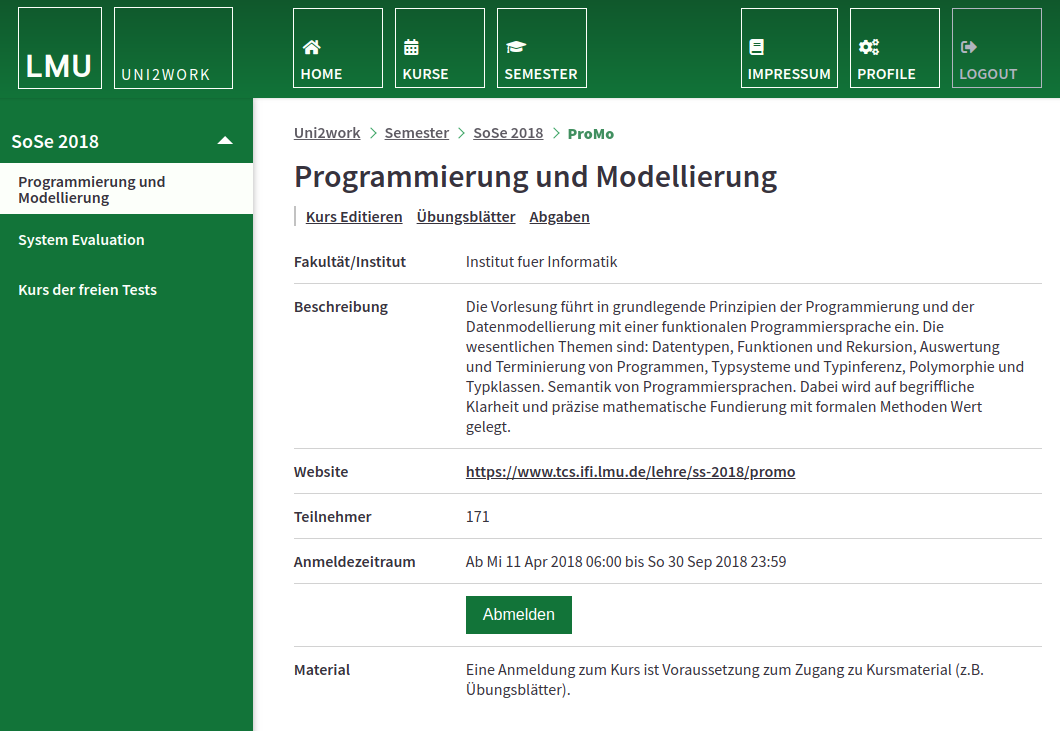
\includegraphics[width=.9\textwidth]{images/uni2work_promo.png}
    \caption{Uni2work -- Die Veranstaltungsseite des Kurses \textit{Programmierung und Modellierung}}
    \label{fig:uni2work_promo}
\end{figure}

\noindent
Der größte Unterschied zu dem Layout des Vorgängers UniWorX liegt in der Navigation der Seiten (vgl. \autoref{fig:uniworx_promo}). In Uni2work wurde die Hauptnavigation am oberen Seitenrand erweitert damit Benutzer schnell zwischen Startseite sowie Veranstaltungs- und Semesterübersicht wechseln können.
Eine Leiste am linken Bildschirmrand beinhaltet in UniWorX sowohl die angemeldeten Veranstaltungen eines Benutzers, als auch die Navigation zu der aktuellen und vergangenen Veranstaltungsübersicht. Diese Navigation wurde in Uni2work in die Hauptnavigation am oberen Seitenrand verschoben, sodass die linke Leiste ausschließlich als Übersicht für angemeldeten Kurse dient. Die Unternavigation die sich bei UniWorX in der Seitenleiste befindet (Übungsgruppen, Abgaben, Klausuren) wurde in Uni2work in den Inhaltsbereich der Seite verlegt, ist jedoch zusätzlich beim Hovern \footnote{Das Verweilen mit dem Mauszeiger über einem Webseiten-Element} über den Einträgen der Seitenleiste erreichbar.

\subsection{Einsatz von JavaScript} \label{sec:einsatz-js}
Um das beinahe vollumfängliche Benutzen der Seite auch ohne JavaScript zu ermöglichen wurde JavaScript ausschließlich für Features eingesetzt die lediglich den Bedienkomfort erhöhen, nicht aber die Funktionalität erweitern um \textit{progressive Verbesserung} zu ermöglichen. Hierbei werden Verbesserungen und neue Features so eingeführt, dass die Webseite auch bei deaktiviertem JavaScript oder anderen Einschränkungen jederzeit benutzbar bleibt. Um die Unterschiede zwischen den geräteabhängigen Erfahrungen der Benutzer so gering wie möglich zu halten wurde sparsam mit JavaScript umgegangen. Insgesamt befinden sich aktuell 880 Zeilen Julius-Code in dem Entwicklungszweig der Anwendung.
Bei der Implementierung wurde sich an wenigen Stellen bewusst dafür entschieden, Benutzern mit aktiviertem JavaScript einige Zusatzfeatures zu bieten deren Fehlen bei deaktiviertem JavaScript die Bedienbarkeit nicht beeinträchtigt.

Als Beispiel seien hier sortierbare Tabellen erwähnt: Der Kopf einer sortierbaren Tabellenspalte dient als Umschalter zwischen auf- und absteigender Sortierung. Dies ist durch zwei entgegengesetzte Pfeile angedeutet, wie in \autoref{fig:sortable_tables} dargestellt. Die ganze Zelle des Tabellenkopfes ist ein Link (\lstinline{<a href="...">}), welcher beim Klicken für Benutzer mit aktiviertem JavaScript die Sortierung asynchron vornimmt, ohne ein komplettes Neuladen der Seite. Ohne JavaScript führt der selbe Link auf die gleiche Seite mit entsprechend sortierter Tabelle. Neben der Einsparung von herunterzuladenen Webseitendaten spart sich der Benutzer somit bei aktiviertem JavaScript auch etwas Zeit bei der Bedienung.

\begin{figure}[h]
    \centering
    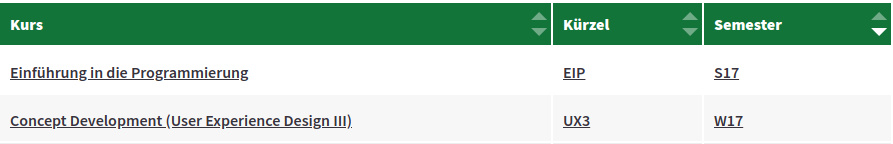
\includegraphics[width=\textwidth]{images/sortable_tables.png}
    \caption{Uni2work -- Sortierbare Tabellenspalten sind im Tabellenkopf durch entgegengesetzte Pfeile am rechten Zellenrand gekennzeichnet.}
    \label{fig:sortable_tables}
\end{figure}

\noindent
Ein weiteres Beispiel sind \textit{Tooltips} die an diversen Orten auf der Seite zum Einsatz kommen und beispielsweise nähere Informationen zu Formularfelder beinhalten, gezeigt in \autoref{fig:uni2work-tooltip}. Diese Tooltip werden erst sichtbar wenn der Benutzer 300 Millisekunden mit dem Mauszeiger über dem entsprechenden Fragezeichen verweilt ("`Hovern"'). Auf Geräten mit Touch-Eingabe wie Smartphones, Tablets erscheint der Tooltip wenn das Fragezeichen vom Benutzer angetippt wurde. Bei fehlendem Javascript passiert nichts bei der Interaktion mit dem Fragezeichen, der Tooltip bleibt für den Benutzer verborgen.

\begin{figure}[H]
    \centering
    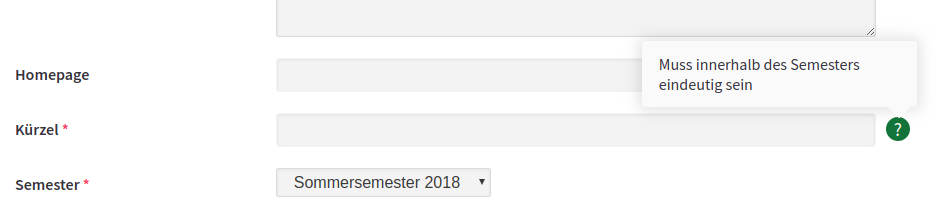
\includegraphics[width=\textwidth]{images/tooltip.png}
    \caption{Uni2work -- Eine Formular-Zeile in Uni2work mit sichtbarem Tooltip}
    \label{fig:uni2work-tooltip}
\end{figure}

\subsection{Bedienbarkeit auf mobilen Endgeräten}
Studien zeigen, dass etwa seit Ende des Jahres 2016 die Besucherzahlen von Internet-Seiten durch mobile Endgeräte (Smartphones und Tablets) diejenigen von Desktop-Rechnern und Laptops übersteigen \cite{web:stonetemple-mobile,web:statcounter-mobile}. Spätestens die Auswertung der Nutzer-Studie zu dieser Arbeit in \autoref{sec:userstudies} zeigt, dass die Bedienbarkeit eines Systems wie UniWorX auf mobilen Endgeräten heutzutage von der Mehrheit der Benutzer gewünscht wird.

UniWorX ist in keiner Hinsicht für kleine Bildschirme optimiert, wodurch vor allem die Navigation auf der Seite erschwert wird. Den richtigen Seitenausschnitt zu finden ist oft mit aufwendigem Zoomen und Scrollen verbunden. In \autoref{fig:mobile_comparison_uniworx} findet sich ein Screenshot des bestehenden Systems UniWorX wie es etwa auf einem iPhone 6 angezeigt wird. UniWorX wird auf dem Smartphone so dargestellt wie es auch auf einem Desktop-Rechner mit größerem Bildschirm dargestellt wird. Um die gesuchten Informationen zu finden müssen hier zwangsläufig Bereiche vom Benutzer vergrößert werden.
\autoref{fig:mobile_comparison_uni2work} zeigt die gleiche Seite in Uni2work.

Gemäß einer offiziellen Empfehlung Microsofts und anderer etablierter Softwarehäuser haben Schaltflächen und klickbare Elemente in Uni2work mindestens die Größe eines Quadrats der Kantenlänge 48 Pixel \cite{web:microsoft-guidelines}\cite{web:apple-guidelines}. Dies entspricht auf einem Bildschirm mit einem Device Pixel Ratio (DPR) von 1 einer Kantenlänge von 9mm \footnote{DPR: Verhältnis zwischen den logischen und den physikalisch verfügbaren Pixeln auf einem Bildschirm.\\DPR von 1 bedeutet, dass die Anzahl der berechneten Pixel der Anzahl der phsyikalisch verügbaren Pixel entspricht.}.

\begin{figure}[h]
    \begin{subfigure}{.49\textwidth}
      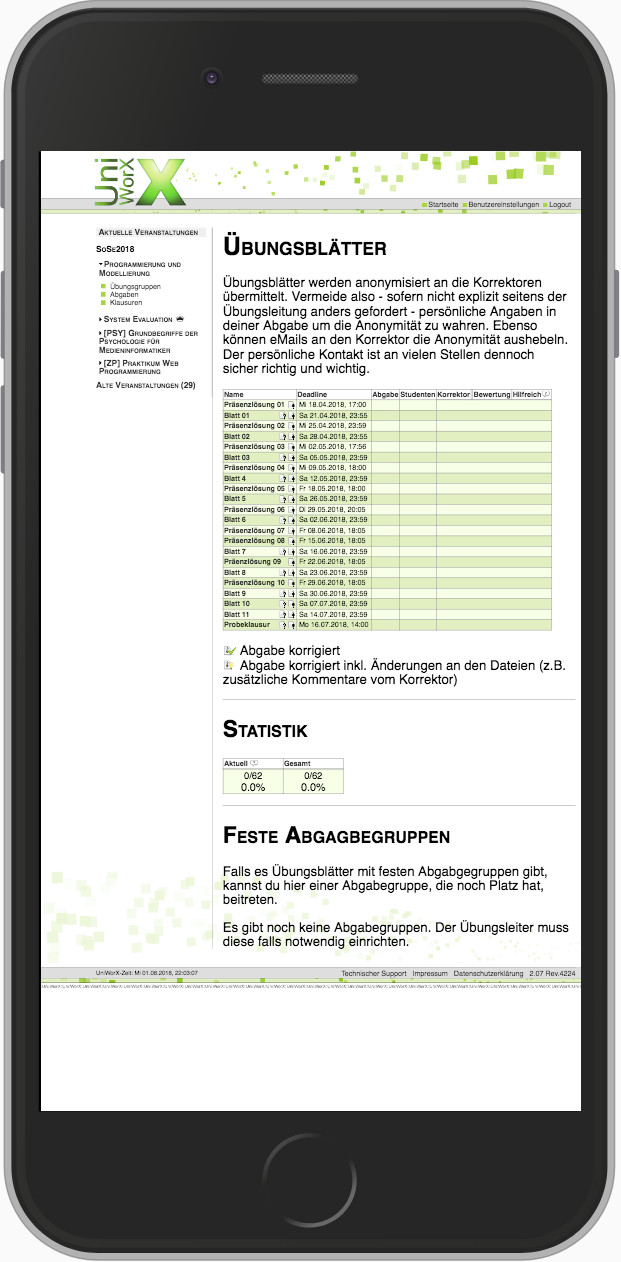
\includegraphics[width=66mm]{images/m_uniworx_sheets.jpg}
      \caption{\textit{UniWorX} \\ Um den Inhalt der Seite lesen oder gezielt auf einen Menüpunkt klicken zu können muss zwangsläufig herangezoomed und gescrolled werden \\ }
      \label{fig:mobile_comparison_uniworx}
    \end{subfigure}
    \hfill
    \begin{subfigure}{.49\textwidth}
      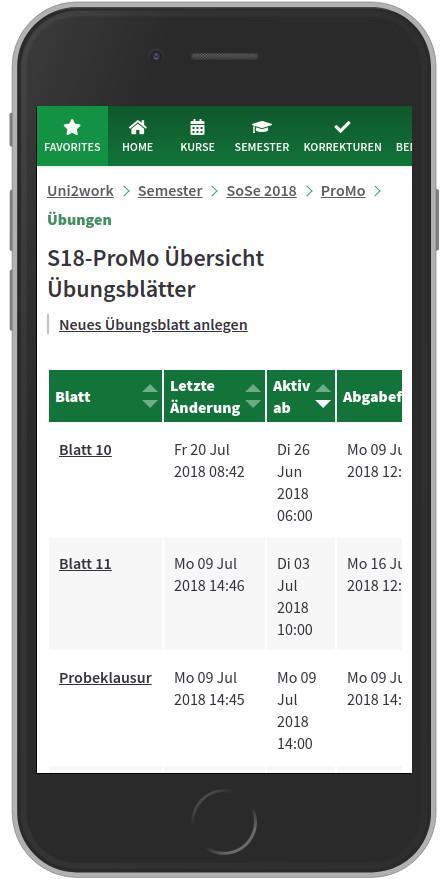
\includegraphics[width=67mm]{images/m_uni2work_sheets_green.jpg}
      \caption{\textit{Uni2work} \\ Benutzeroberfläche angepasst für kleine Bildschirme. Die Navigation am oberen Bildschirmrand und die Tabelle mit den Abgaben können seitwärts gescrolled werden.}
      \label{fig:mobile_comparison_uni2work}
    \end{subfigure}
    \caption{Links UniWorX -- Rechts Uni2work.\\Übersicht abgegebener Übungsblatt-Lösungen für den Kurs ProMo auf einem Iphone 6.}
    \label{fig:mobile_comparison}
\end{figure}

\noindent
Die Seitenleiste die in \autoref{sec:uni2work_user-interface} etwas genauer vorgestellt wurde stellt ein Feature dar, das auf großen Bildschirmen stets erreichbar ist. Auf mobilen Geräten mit kleinen Bildschirmen wurde diese Leiste aus dem dauernden Seitenbild entfernt und ist dort stattdessen nur bei Bedarf sichtbar. In \autoref{fig:uni2work_mobile_favorites} ist diese Leiste zu sehen, sowie der \textit{Favorites}-Button in der Hauptnavigation der zwischen sichtbaren und versteckten Favoriten umschaltet.

\begin{figure}
    \begin{subfigure}{.49\textwidth}
      
\includegraphics[width=67mm]{images/m_uni2work_promo_favorites_hidden.jpg}
      \caption{Favoriten versteckt}
      \label{fig:uni2work_fav_hid}
    \end{subfigure}%
    \hfill
    \begin{subfigure}{.49\textwidth}
      
\includegraphics[width=67mm]{images/m_uni2work_promo_favorites_visible.jpg}
      \caption{Favoriten sichtbar}
      \label{fig:uni2work_fav_vis}
    \end{subfigure}
    \caption{Favoriten-Leiste öffnet und schließt sich bei Bedarf durch Antippen des \textit{Favorites}-Buttons in der Hauptnavigation.}
    \label{fig:uni2work_mobile_favorites}
\end{figure}

\subsection{Barrierefreiheit}
Um allen zukünftigen Benutzern den Umgang mit Uni2work zu ermöglichen wurden grundlegende Vorkehrungen für die Barrierefreiheit getroffen. Klare Farbkontraste und angemessene Abstände (Gestaltgesetze \footnote{Gesetz der Nähe, Gesetz der Ähnlichkeit, \cite{web:wikigestalt}}) sollen visuell Beeinträchtigten die Bedienung erleichtern. Für blinde Benutzer wurde das leichte Einpflegen von entsprechenden HTML-Attributen für Screen Reader \footnote{Software die den Inhalt einer Webseite (oder eines beliebigen Programms) vorlesen oder anderweitig zugänglich machen kann} vorbereitet. Näheres hierzu in \autoref{sec:future_work}.

\clearpage
\section{Evaluation} \label{sec:userstudies}
Neben der Implementierung des Systems Uni2work soll im Rahmen dieser Arbeit die Bedienbarkeit des neuen Systems evaluiert werden. Hierfür wurde eine Studie mit den Benutzern des Vorgängers UniWorX durchgeführt. Im Zuge der Studie wurden die Teilnehmer (siehe \autoref{sec:studyparticipants}) aufgefordert entweder das alte System (UniWorX) oder das neue System (Uni2work) für eine realitätsnahe Aufgabe aus dem studentischen Alltag zu verwenden, um sowohl Messdaten über das alte als auch das neue System zu erhalten. In den folgenden Unterabschnitten soll auf die angewandte Methode, die Studienteilnehmer und weitere Details der Studie eingegangen werden.

\subsection{Methode} \label{sec:method}
In der Zeit vom 01.07.2018 bis zum 24.07.2018 wurde eine Studie in Form eines Online-Fragebogens in englischer Sprache durchgeführt.
Das Ziel des Studie war es die Usability von UniWorX und Uni2work zu evaluieren um einerseits auf die Kritik an UniWorX eingehen zu können und andererseits frühe Fehler in der Entwicklung von Uni2work zu vermeiden. Als Plattform für die Einrichtung und Verbreitung des Fragebogens wurde \textit{Google Forms} \footnote{\url{https://forms.google.com}} gewählt. Der Fragebogen wurde im angegebenen Zeitraum 146 mal ausgefüllt.

Unter den gesammelten Beobachtungen ließen sich beim manuellen Sichten der Daten 11 Datenpunkte identifizieren die für die weitere Analyse entfernt wurden, da sie jegliches qualitatives Feedback vermissen ließen und auf alle gestellten Fragen gleich antworteten.

Bei der Studie handelte es sich um eine \emph{"`within subjects"'}-Studie bei der Teilnehmer der Studie den gleichen Fragebogen auf freiwilliger Basis ein zweites Mal ausfüllen konnten. Die Teilnehmer mussten zu Beginn des Fragebogens eine Aufgabe erfüllen für die sie entweder das bereits vertraute UniWorX (siehe \autoref{sec:uniworx}) oder das neue Uni2work benutzen sollten. Ein Teil der anschließenden Fragen bezog sich dann -- soweit nicht anders angegeben -- auf das System das für diese einleitende Aufgabe benutzt wurde. Nach vollständigem Beantworten des Fragebogens wurden die Teilnehmer gebeten den Fragebogen erneut auszufüllen, jedoch bei der anfänglichen Aufgabe das jeweils andere System zu wählen. Den Teilnehmern entstand kein Vorteil durch das zweimalige Ausfüllen des Fragebogens und es wurde nicht erhoben wie viele der Teilnehmer den Fragebogen tatsächlich mehrmals ausgefüllt haben.

Die durch den Fragebogen gesammelten Beobachtungen lassen sich demnach in zwei Gruppen aufteilen, welche sich lediglich in dem für die initiale Aufgabe benutzten System unterscheiden. Somit existiert unter den Messdaten ausschließlich \emph{eine unabhängige Variable}:

\begin{itemize}
    \item \textbf{Gruppe UniWorX} hat das System \textbf{UniWorX} für die Aufgabe benutzt und evaluiert.
    \item \textbf{Gruppe Uni2work} hat das System \textbf{Uni2work} für die Aufgabe benutzt und evaluiert.
\end{itemize}

\noindent
Für die folgenden Unterabschnitte ist ein Verständnis der Likert-Skala nötig. Hierfür soll nun knapp auf diese Skala eingegangen werden. Anschließend wird der in dieser Studie eingesetzte System Usability Scale beschrieben.

\subsection{Likert-Skala} \label{sec:likert}

Die Likert-Skala bietet die Möglichkeit die Einstellung einer Person zu bestimmten Themen zu messen. Eine Likert-Skala besteht aus mehreren Aussagen des Likert-Typs. Eine solche Aussage muss eine bedeutungsvolle Reaktion zwischen "`trifft nicht zu"' und "`trifft zu"' zulassen \footnote{Bedeutungslos wäre eine solche Reaktion z.B. für die Aussage "`Deine Reaktion ist mir egal."'}. Üblicherweise beinhaltet die Antwortskala für die Reaktion eines Teilnehmers 4, 5 oder 7 Abstufungen. \autoref{fig:likert-scale-question} stellt dar, wie eine solche Aussage in dem eingesetzten Fragebogen ausgesehen hat.

\begin{figure}[h]
    \centering
    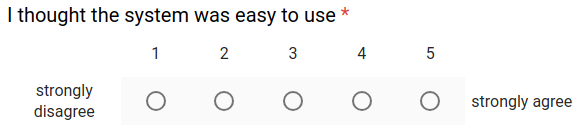
\includegraphics[width=.8\textwidth]{images/likert-scale.png}
    \caption{Eine Aussage des Likert-Typs als "`Frage"' in dem eingesetzten Fragebogen}
    \label{fig:likert-scale-question}
\end{figure}

\subsection{System Usability Scale (SUS)} \label{sec:sus}
Der \emph{System Usability Scale} (SUS) wurde 1986 von John Brooke veröffentlicht. Er besteht aus zehn standardisierten Aussagen die mit der Antwortskala der Likert-Skala zu beantworten sind. Die Reaktionen auf diese zehn Aussagen werden zu einem genormten Wert zwischen 0 und 100 umgerechnet und erlauben somit einen vergleichbaren Messwert der gefühlten Usability eines Systems.

Mit Hilfe des SUS können Systeme domäneübergreifend auf ihre Bedienbarkeit untersucht werden indem die enthaltenen Aussagen nicht auf spezielle Funktionalitäten des \emph{System Under Test} (\emph{SUT} -- das System das getestet wird) eingehen, sondern die Einstellung der Teilnehmer zu generellen Aspekten der Usability messen.

\begin{quote}
\emph{"'[...] there are no absolute measures of usability [...]"'} -- John Brooke, \cite{brooke_sus}
\end{quote}
"`Usability ist nicht in absoluten Werten messbar"'. Mit dieser Aussage unterstreicht der Erfinder des SUS, John Brooke, dass ein einzelner Wert dieser Skala keine Aussagekraft besitzt. Erst der Vergleich mit Werten unterschiedlicher Systeme (in diesem Fall: UniWorX und Uni2work) bringt einen tatsächlichen Informationsgewinn. \cite{brooke_sus}

In der mit dieser Arbeit verbundenen Studie sollte die Usability des neuen Uni2works mit der Usability des bestehenden UniWorX verglichen werden. Für diesen Zweck eignet sich der SUS als standardisierter Test und wurde wegen seiner großen Verbreitung und Bekanntheit verwendet.

\paragraph{Die zehn standardisierten Aussagen des SUS}  \hfill \\
(mit vorangestellten Identifikatoren Q1-Q10 für spätere Referenzierung)

\begin{itemize}
    \item \textbf{Q1: Ich denke ich würde dieses System gerne oft benutzen} \\ ("'I think that I would like to use this system frequently"')
    \item \textbf{Q2: Ich fand das System unnötig komplex} \\ ("'I found the system unnecessarily complex"')
    \item \textbf{Q3: Ich fand das System einfach zu benutzen} \\ ("'I thought the system was easy to use"')
    \item \textbf{Q4: Ich denke ich würde technische Hilfe in Anspruch nehmen müssen um das System zu benutzen} \\ ("'I think that I would need the support of a technical person to be able to use this system"')
    \item \textbf{Q5: Ich fand die verschiedenen Funktionen des Systems waren gut integriert} \\ ("'I found the various functions in this system were well integrated"')
    \item \textbf{Q6: Ich fand es gab zu viele Inkonsistenzen in dem System} \\ ("'I thought there was too much inconsistency in this system"')
    \item \textbf{Q7: Ich kann mir vorstellen, dass die meisten Menschen den Umgang mit dem System sehr schnell lernen könnten} \\ ("'I would imagine that most people would learn to use this system very quickly"')
    \item \textbf{Q8: Ich empfand die Benutzung des Systems als sehr mühsam} \\ ("'I found the system very cumbersome to use"')
    \item \textbf{Q9: Ich habe mich sehr sicher beim Umgang mit dem System gefühlt} \\ ("'I felt very confident using the system"')
    \item \textbf{Q10: Ich musste viel lernen bevor ich mit dem System umzugehen wusste} \\ ("'I needed to learn a lot of things before I could get going with this system"')
\end{itemize}

\noindent
Eine Formel übersetzt die vorgestellten Reaktionen der Studienteilnehmer auf die SUS-Aussagen in einen einzelnen SUS-Wert. Bei ungeraden Aussagen (Aussage 1, Aussage 3, ...) führt Zustimmung, bei geraden Aussagen (Aussage 2, Aussage 4, ...) Ablehnung zu einem besseren End-Wert \cite{brooke_sus}.

\subsection{Studienteilnehmer} \label{sec:studyparticipants}
Bei den Teilnehmern dieser Studie handelte es sich ausschließlich um Besucher der Veranstaltung "`Programmierung und Modellierung"' bei Dr. Steffen Jost im Sommersemester 2018.

Der Link zu dem Online-Fragebogen wurde auf einem Übungsblatt des Kurses "`Programmierung und Modellierung"' veröffentlicht. Als Motivation zur Beantwortung des Fragebogens wurden den Teilnehmern Bonuspunkte im Übungsbetrieb gewährt. Es erhielten jedoch nur diejenigen Teilnehmer Bonuspunkte welche die initiale Aufgabe des Fragebogens (s. \autoref{sec:study_structure}) erfolgreich abgeschlossen haben. Im Rahmen dieser Aufgabe mussten die Teilnehmer eine Abgabe über das von ihnen gewählte System hochladen. Obwohl nicht direkt erfasst wurde wie viele der für die 146 Antworten verantwortlichen Teilnehmer den Fragebogen ein zweites Mal ausgefüllt haben, kann über die Anzahl der eingereichten Arbeiten davon ausgegangen werden, dass 89 unterschiedliche Personen an der Studie teilgenommen haben.

\subsection{Fragebogenstruktur} \label{sec:study_structure}
Der Fragebogen war in sieben Sektionen aufgeteilt, welche hier im Detail erläutert werden.

\subsubsection{Sektion 1: Generelle Fragen zur Person}
Die Fragen in dieser Sektion sollten den Teilnehmer auf die Situation vorbereiten und langsam an das Befragt-Werden gewöhnen. Die Teilnehmer wurden gebeten ihr Alter und ihre ungefähre Nutzungshäufigkeit von UniWorX anzugeben. Da alle Studenten die an der Studie teilgenommen haben zwangsläufig UniWorX für ihren Studienalltag benutzen müssen konnte hier davon ausgegangen werden, dass alle Teilnehmer mit UniWorX vertraut waren.

Auf die Frage \textbf{"`Wie oft benutzen Sie UniWorX ungefähr?"'} konnte mit einer dieser sechs Möglichkeiten geantwortet werden:

\begin{itemize}
    \item \textbf{Einmal pro Semester} \\ ("`Once a term"')
    \item \textbf{Einmal pro Monat} \\ ("`Once a month"')
    \item \textbf{Einmal pro Woche} \\ ("`Once a week"')
    \item \textbf{Bis zu fünf Mal pro Woche} \\ ("`Up to five times a week"')
    \item \textbf{Täglich} \\ ("`Daily"')
    \item \textbf{Andauernd} \\ ("`All the time"')
\end{itemize}

\bigskip
\noindent
Für die Angabe des \textbf{Alters} wurde ein Textfeld dargeboten.

\subsubsection{Sektion 2: Task}
In dieser Sektion wurde der Teilnehmer aufgefordert eine Aufgabe zu erledigen und die Beantwortung des Fragebogens erst nach beendeter Durchführung der Aufgabe fortzusetzen.

Die genaue Aufgabenstellung in englischer Sprache lautete 
\begin{quote}
\itshape 
Please complete this task before you proceed with this questionnaire:

Use either UniWorX OR Uni2work to find the course "'System Evaluation"' and register for it!
Once you are registered submit anything for the sheet "'Submission Evaluation"'.

UniWorX: https://uniworx.ifi.lmu.de
Uni2work: https://uni2work.ifi.lmu.de

Continue with this questionnaire afterwards.
\end{quote}

\noindent
Eine freie Übersetzung ins Deutsche:
\begin{quote}
\itshape
Bitte beenden Sie diese Aufgabe bevor Sie mit dem Beantworten des Fragebogens fortfahren:

Benutzen Sie \textbf{entweder} UniWorX \textbf{oder} Uni2work um den Kurs "`System Evaluation"' zu finden und sich für den Kurs zu registrieren.
Wenn Sie sich erfolgreich angemeldet haben laden Sie eine beliebige Datei als Abgabe für das Übungsblatt "`Submission Evaluation"' hoch.

[Links zu den beiden Systemen UniWorX und Uni2work]

Fahren Sie im Anschluß mit der Beantwortung dieses Fragebogens fort.
\end{quote}

\subsubsection{Sektion 3: Wahl des Systems}
In dieser Sektion sollte der Teilnehmer lediglich angeben für welches System er sich im vorangegangenen Schritt entschieden hat.

\subsubsection{Sektion 4: Usability des Systems}
Je nach dem System welches der Teilnehmer in Sektion 2 gewählt hat, wurden ihm in dieser Sektion die zehn Aussagen des SUS für das entsprechende System als Likert-Skala präsentiert.

\subsubsection{Sektion 5: Spezifischere Fragen zum System}
Nach den stark standardisierten Aussagen des SUS in der vorangegangen Sektion wurden in dieser Sektion etwas spezifischere Aussagen dargeboten die auf die Eigenheiten der Systeme eingehen sollten. Diese vier Aussagen wurden ebenfalls als Likert-Skala präsentiert.

\begin{itemize}
    \item \textbf{Ich konnte das System eindeutig der LMU zuordnen} \\ ("'I clearly recognized the system as a part of the LMU"')
    \item \textbf{Ich konnte mich sehr einfach zu einem Kurs anmelden} \\ ("'I was able to register for a course very easily"')
    \item \textbf{Ich konnte das Formular zum Hochladen einer Abgabe schnell finden} \\ ("'I was able to find the form for the sheet submission quickly"')
    \item \textbf{Es war offensichtlich ob meine Aktionen erfolgreich waren} \\ ("'It was very obvious whether or not my actions were successful"')
\end{itemize}

\subsubsection{Sektion 6: Freie Meinungen}
Unter dem Titel "'Other opinions"' konnte der Teilnehmer in dieser Sektion seine Meinungen zu dem benutzten System in Textform äußern. Es wurden Textfelder für folgende Fragen geboten:

\begin{itemize}
    \item \textbf{Was hat Ihnen \emph{besonders gut} gefallen?} \\ ("'Did you like something in particular?"')
    \item \textbf{Was hat Ihnen \emph{besonders schlecht} gefallen?} \\ ("'Did you dislike something in particular?"')
    \item \textbf{Was würden Sie verbessern?} \\ ("'What would you improve?"')
    \item \textbf{Falls Sie das andere System bereits benutzt haben: Was würden Sie daran verbessern?} \\ ("'You feel like you can contribute something to the other system?"')
\end{itemize}

\noindent
Nach diesen vier Freitextfragen wurde der Teilnehmer gefragt ob er ein solches System gerne auch auf mobilen Endgeräten verweden würde. Hat der Teilnehmer auf diese Frage mit "`Nein"' geantwortet so wurde er ans Ende des Fragebogens geleitet.

\subsubsection{Sektion 7: Usability auf mobilen Endgeräten (Optional)}
Teilnehmer die in der vorigen Sektion angegeben haben, dass sie an einer Benutzung des Systems auf mobilen Endgeräten interessiert wären wurden hier zu ihrem Verhalten auf diesen Geräten befragt.

\begin{itemize}
    \item \textbf{Wie oft besuchen Sie Webseiten die mit Ihrer Universität in Verbindung stehen auf Ihrem Handy oder ähnlichem Gerät?} \\ ("'How often do you visit university related websites on your phone or a similar mobile device?"') \\
    \emph{Antwortmöglichkeiten:}
        
    \begin{itemize}
        \item \textbf{Einmal pro Semester} \\ ("`Once a term"')
        \item \textbf{Einmal pro Monat} \\ ("`Once a month"')
        \item \textbf{Einmal pro Woche} \\ ("`Once a week"')
        \item \textbf{Bis zu fünf Mal pro Woche} \\ ("`Up to five times a week"')
        \item \textbf{Täglich} \\ ("`Daily"')
        \item \textbf{Andauernd} \\ ("`All the time"')
    \end{itemize}
    
    \item \textbf{Haben Sie UniWorX jemals mit Ihrem Handy besucht?} \\ ("'Did you use UniWorX on your mobile device in the past?"') \\ \emph{Antwortmöglichkeiten:} \\ \textbf{Ja | Nein | Vielleicht}
    
    \item \textbf{Würden Sie UniWorX mehr benutzen wenn es besser an kleine Bildschirme angepasst wäre?} \\ ("'Would you use UniWorX more often on your mobile device if it was better suited for small screens?"') \\ \emph{Antwortmöglichkeiten:} \\ \textbf{Ja | Nein | Vielleicht | Habe es nicht benutzt}
\end{itemize}

\noindent
Nach diesen Fragen kam eine weitere, optionale Freitext-Frage für besonders engagierte Teilnehmer die mit \textbf{"'Feeling extra helpful?"'} angesprochen wurden. Diese wurden gebeten mit einem mobilen Gerät ihrer Wahl durch Uni2work zu navigieren und dann ihre freie Meinung zu dem System in Text-Form zu äußern.

\clearpage
\section{Ergebnisse}
In den folgenden Unterabschnitten werden die Umfrageergebnisse und deren Auswertung betrachtet.

\subsection{Demographie}
Die Teilnehmer der Studie waren im Mittel 22 Jahre alt (Gruppe UniWorX: 22,4, Gruppe Uni2work: 21,6). Weitere persönliche Daten wurden nicht erfasst.
\autoref{fig:usage-pie} zeigt wie häufig die Teilnehmer UniWorX benutzen. Über 98\% der Teilnehmer benutzen das System mindestens ein Mal pro Woche.
Die Teilnahme an der Studie war freiwillig. Das lässt vermuten, dass insbesondere Studenten die UniWorX oft benutzen gewillt waren an dieser Umfrage teilzunehmen um Einfluss auf den Nachfolger zu haben. Es ist demnach nicht auszuschließen, dass die tatsächliche Nutzungshäufigkeit etwas unter dem ermittelten Wert liegt. Unabhängig von dem potentiellen Einfluss auf das Ergebnis der Frage nach der Nutzungshäufigkeit, verleiht das Ergebnis der Notwendigkeit eines stabilen und wartbaren Systems Ausdruck.

\begin{figure}[h]
    \centering
    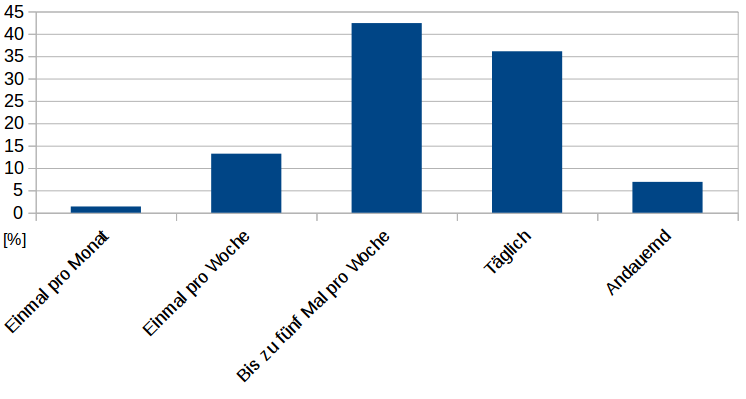
\includegraphics[width=\textwidth]{images/uniworx_usage.png}
    \caption{Die Nutzungshäufigkeit von UniWorX}
    \label{fig:usage-pie}
\end{figure}

\subsection{System Usability Scale (SUS)} \label{sec:results_sus}
In \autoref{fig:results_sus} sind die Teilnehmerreaktionen auf die SUS-Aussagen gegenübergestellt. Die Verteilungen der Reaktionen stimmen bei beiden System weitestgehend überein, bei UniWorX ist jedoch ein ausgeprägterer Trend zu den Extremen hin erkennbar. In \autoref{fig:results_sus} ist das an den tendenziell größeren hellblauen und dunkelblauen Flächen bei UniWorX im Vergleich zu Uni2work erkennbar. Lediglich auf die SUS-Aussagen 4, 5 und 8 reagierten die Benutzer des Systems Uni2work mit eindeutigeren Werten als die des Systems UniWorX, d.h. die relative Häufigkeit der Reaktionen abseits der neutralen Mitte war häufiger.

\begin{figure}[H]
    \centering
    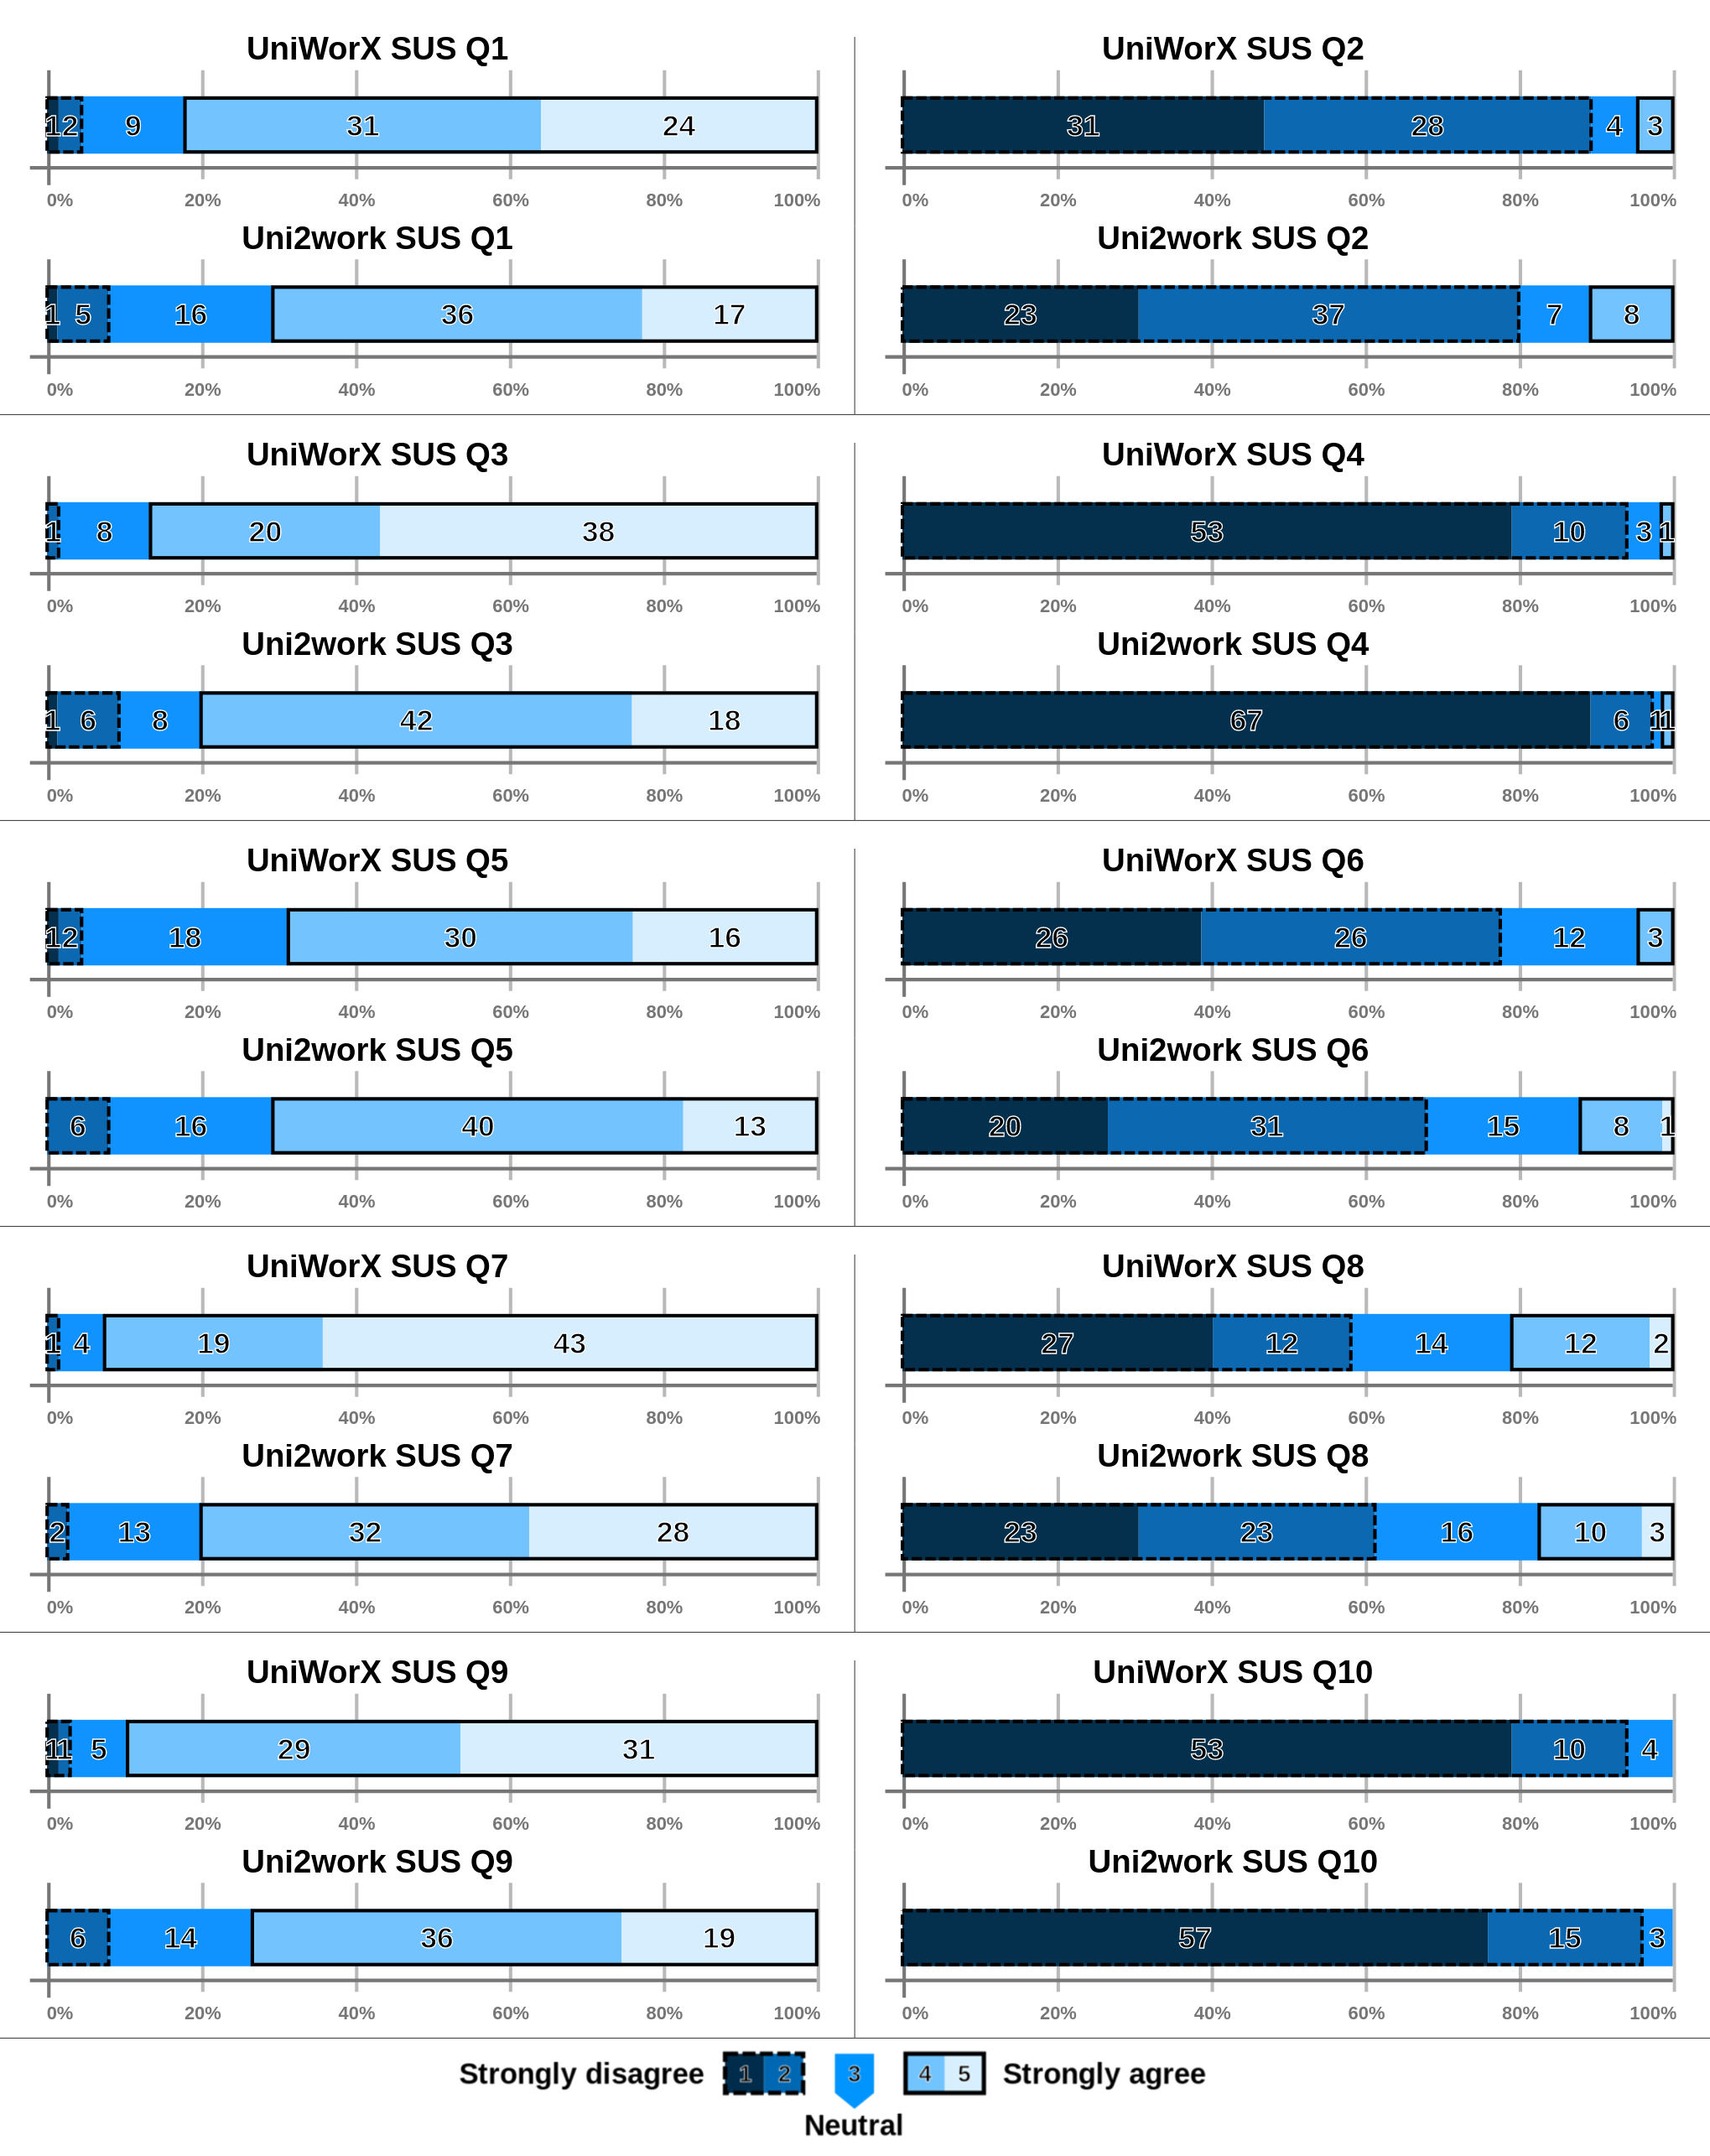
\includegraphics[width=\textwidth]{images/likert_comparison.jpg}
    \caption{Vergleich der SUS-Reaktionen. Zahlen in den farbigen Flächen stellen absolute Häufigkeiten dar. Q1-Q10 entsprechen den in \autoref{sec:sus} vorgestellten Aussagen des SUS.}
    \label{fig:results_sus}
\end{figure}

\noindent
Es sollen nun die Reaktionen auf die einzelnen Aussagen detaillierter betrachtet werden:

\begin{itemize}
    \item \textbf{Q1: Ich denke ich würde dieses System gerne öfter benutzen}
    
    \smallskip
    \begin{tabular}{p{6.5cm}|p{6.5cm}}
        \textit{UniWorX} & \textit{Uni2work} \\
        82\% stimmten dieser Aussage zu & 71\% stimmten dieser Aussage zu \\
        4\% widersprachen dieser Aussage & 8\% widersprachen dieser Aussage \\
        (14\% verhielten sich neutral) &  (21\% verhielten sich neutral)
    \end{tabular}
    
    \smallskip
    Der Unterschied zwischen den Benutzergruppen lässt sich damit erklären, dass die Benutzer bereits vertraut im Umgang mit UniWorX waren und eine Zustimmung somit leichter fiel. Da die Teilnehmer der Uni2work-Gruppe zu dem Zeitpunkt der Fragestellung das System lediglich für wenige Minuten benutzt hatten war die initiale menschliche Scheu vor Neuem und Unbekanntem noch nicht überwunden, wodurch insgesamt weniger Teilnehmer dieser Aussage zustimmten.
    \item \textbf{Q2: Ich fand das System unnötig komplex}
    
    \smallskip
    \begin{tabular}{p{6.5cm}|p{6.5cm}}
        \textit{UniWorX} & \textit{Uni2work} \\
        4\% stimmten dieser Aussage zu & 11\% stimmten dieser Aussage zu \\
        89\% widersprachen dieser Aussage & 80\% widersprachen dieser Aussage \\
        (7\% verhielten sich neutral) &  (9\% verhielten sich neutral)
    \end{tabular}
    
    \smallskip
    Die Bekanntheit der VLE UniWorX unter den Teilnehmern und das bis dato gewonnenene Vertrauen in jenes System spielten sicher eine Rolle bei dem Unterschied zwischen den Reaktionen der beiden Benutzergruppen auf diese Aussage.
    \item \textbf{Q3: Ich fand das System einfach zu benutzen}
    
    \smallskip
    \begin{tabular}{p{6.5cm}|p{6.5cm}}
        \textit{UniWorX} & \textit{Uni2work} \\
        86\% stimmten dieser Aussage zu & 80\% stimmten dieser Aussage zu \\
        1\% widersprachen dieser Aussage & 9\% widersprachen dieser Aussage \\
        (13\% verhielten sich neutral) &  (11\% verhielten sich neutral)
    \end{tabular}
    
    \smallskip
    Auch bei dieser Aussage spielte die Bekanntheit von UniWorX sicher eine Rolle. Die Teilnehmer der Studie benutzten zu dem Zeitpunkt der Umfrage das System UniWorX bereits seit mehreren Semestern und haben gelernt mit den Mängeln umzugehen.
    \item \textbf{Q4: Ich denke ich würde technische Hilfe in Anspruch nehmen müssen um das System zu benutzen}
    
    \smallskip
    \begin{tabular}{p{6.5cm}|p{6.5cm}}
        \textit{UniWorX} & \textit{Uni2work} \\
        1\% stimmten dieser Aussage zu & 1\% stimmten dieser Aussage zu \\
        94\% widersprachen dieser Aussage & 97\% widersprachen dieser Aussage \\
        (5\% verhielten sich neutral) &  (2\% verhielten sich neutral)
    \end{tabular}
    
    \smallskip
    Beide Systeme scheinen laut den Studienteilnehmern sehr intuitiv in ihrer Bedienung zu sein. Der Unterschied zwischen den Gruppen ist vernachlässigbar.
    \item \textbf{Q5: Ich fand die verschiedenen Funktionen des Systems waren gut integriert}
    
    \smallskip
    \begin{tabular}{p{6.5cm}|p{6.5cm}}
        \textit{UniWorX} & \textit{Uni2work} \\
        69\% stimmten dieser Aussage zu & 71\% stimmten dieser Aussage zu \\
        4\% widersprachen dieser Aussage & 8\% widersprachen dieser Aussage \\
        (27\% verhielten sich neutral) &  (21\% verhielten sich neutral)
    \end{tabular}
    
    \smallskip
    Der unterdurchschnittliche Grad an Zustimmung unter den UniWorX-Benutzern im Vergleich zu den anderen Aussagen weist auf Mängel in der Usability hin. Unter schlecht integrierten Funktionen sind Funktionen zu verstehen die zwar zweckmäßig sind, jedoch an Stellen im System verborgen liegen an denen sie nicht vermutet werden. Die Teilnehmer der Uni2work-Gruppe haben das System Uni2work zu dem Zeitpunkt der Studie lediglich für wenige Minuten benutzt, womit die Bedeutung der etwas höheren Zustimmung aus dieser Gruppe keine allzu große Beachtung geschenkt werden sollte. Eine fundierte Meinung zu dieser Aussage stellt sich erst nach ausgiebiger Benutzung ein. Der Unterschied zwischen den Gruppen ist demnach vernachlässigbar.
    \item \textbf{Q6: Ich fand es gab zu viele Inkonsistenzen in dem System}
    
    \smallskip
    \begin{tabular}{p{6.5cm}|p{6.5cm}}
        \textit{UniWorX} & \textit{Uni2work} \\
        4\% stimmten dieser Aussage zu & 12\% stimmten dieser Aussage zu \\
        78\% widersprachen dieser Aussage & 68\% widersprachen dieser Aussage \\
        (18\% verhielten sich neutral) &  (20\% verhielten sich neutral)
    \end{tabular}
    
    \smallskip
    Ein Großteil des fehlenden Widerspruchs auf Seiten der Uni2work-Benutzer rührt sicherlich daher, dass Uni2work zum Zeitpunkt der Studie in einer frühen Beta-Phase war und es durchaus eindeutige Inkonsistenzen gab. Beispielsweise unterschieden sich manche Tabellen optisch drastisch von anderen Tabellen im System. Da Tabellen eines der Haupt-Instrumente zur Darstellung von Daten in Uni2work sind waren die Unterschiede hier eindeutig und erhöhten den Eindruck der Inkonsistenzen im System spürbar.
    \item \textbf{Q7: Ich kann mir vorstellen, dass die meisten Menschen den Umgang mit dem System sehr schnell lernen könnten}
    
    \smallskip
    \begin{tabular}{p{6.5cm}|p{6.5cm}}
        \textit{UniWorX} & \textit{Uni2work} \\
        93\% stimmten dieser Aussage zu & 80\% stimmten dieser Aussage zu \\
        1\% widersprachen dieser Aussage & 3\% widersprachen dieser Aussage \\
        (6\% verhielten sich neutral) &  (17\% verhielten sich neutral)
    \end{tabular}
    
    \smallskip
    Der Unterschied zwischen den Benutzergruppen lässt sich bei dieser Aussage durch die Bekanntheit des Systems UniWorX erklären. Nachdem die UniWorX-Benutzer unter den Studienteilnehmern bereits seit mehreren Semestern mit UniWorX vertraut waren verdrängten sie die anfängliche Unsicherheit im Umgang mit dem System. Verglichen mit den Reaktionen auf Aussage Q4 ist der Unterschied zwischen den Reaktionen der Benutzerguppen bei dieser Aussage dennoch erstaunlich.
    \item \textbf{Q8: Ich empfand die Benutzung des Systems als sehr mühsam}
    
    \smallskip
    \begin{tabular}{p{6.5cm}|p{6.5cm}}
        \textit{UniWorX} & \textit{Uni2work} \\
        21\% stimmten dieser Aussage zu & 17\% stimmten dieser Aussage zu \\
        58\% widersprachen dieser Aussage & 61\% widersprachen dieser Aussage \\
        (21\% verhielten sich neutral) &  (22\% verhielten sich neutral)
    \end{tabular}
    
    \smallskip
    Obwohl die UniWorX-Benutzer bereits vertraut waren mit dem System und daher mit den Mängeln in der Bedienbarkeit umzugehen wissen sollten, haben sie zögerlicher widersprochen als die Uni2work-Benutzer. Insgesamt fielen die Widersprüche auf diese Aussage äußerst zurückhaltend aus. Der kleine Unterschied zwischen den Gruppen von 3 Prozentpunkten wirkt jedoch umso gravierender wenn die Bekanntheit von UniWorX in Betracht gezogen wird. Die Vertrautheit mit UniWorX sollte die scheinbar vorhandene Mühsamkeit zumindest teilweise lindern.
    \item \textbf{Q9: Ich habe mich sehr sicher beim Umgang mit dem System gefühlt}
    
    \smallskip
    \begin{tabular}{p{6.5cm}|p{6.5cm}}
        \textit{UniWorX} & \textit{Uni2work} \\
        90\% stimmten dieser Aussage zu & 73\% stimmten dieser Aussage zu \\
        3\% widersprachen dieser Aussage & 8\% widersprachen dieser Aussage \\
        (7\% verhielten sich neutral) &  (19\% verhielten sich neutral)
    \end{tabular}
    
    \smallskip
    Dieser Unterschied zwischen den beiden Gruppen ist (analog zu Q6) durch die Inkonsistenzen in Uni2work zum Zeitpunkt der Studie zu erklären. Durch die qualitative Auswertung der offenen Fragen (siehe \autoref{sec:results_qualitative}) wurde hier jedoch deutlich, dass tatsächlich wesentliche Vorgänge und Interaktionen im System ausreichendes Feedback für den Benutzer vermissen ließen.
    \item \textbf{Q10: Ich musste viel lernen bevor ich mit dem System umzugehen wusste}
    
    \smallskip
    \begin{tabular}{p{6.5cm}|p{6.5cm}}
        \textit{UniWorX} & \textit{Uni2work} \\
        0\% stimmten dieser Aussage zu & 0\% stimmten dieser Aussage zu \\
        94\% widersprachen dieser Aussage & 96\% widersprachen dieser Aussage \\
        (6\% verhielten sich neutral) &  (4\% verhielten sich neutral)
    \end{tabular}
    
    \smallskip
    Die Sicherheit mit der die Teilnehmer dieser Aussage widersprachen und der geringe Unterschied zwischen den Gruppen verhält sich sehr ähnlich zu Q4. Beide Systeme scheinen etwa gleichermaßen intuitiv bedienbar zu sein und bedürfen keiner weiteren Instruktionen oder gar Schulung.
\end{itemize}

\noindent
Die entsprechend der SUS-Formel resultierenden Werte zwischen 0 und 100 belaufen sich bei UniWorX auf \textbf{82,27} und bei Uni2work auf \textbf{76,8}. Dem bestehenden System UniWorX wurde demnach eine leicht bessere Usability zugesprochen als dem Nachfolger Uni2work. Die in der Diskussion zu diesen Ergebnissen in \autoref{sec:results_discussion} beschriebenen Mängel von Uni2work während der Umfrage sind in der Kombination mit den sehr generell gehaltenen Aussagen des SUS höchstwahrscheinlich nicht zuträglich für die Bewertung von Uni2work. Da die Teilnehmer mit UniWorX vertraut sind ist es wahrscheinlich, dass ihr Eindruck der Usability des Systems positiv verzerrt ist. Dieser \textit{Status Quo Bias} wird ausführlicher in der Diskussion zu diesen Ergebnissen behandelt.

\subsection{Spezifischere Fragen zum System} \label{sec:results_likert}
In Sektion 5 des Fragebogens (s. \autoref{sec:study_structure}) wurden weitere Fragen in Form von Likert-Typ-Aussagen gestellt. Diese Fragen und ihre Antworten lauten:

\begin{itemize}
    \item \textbf{Ich konnte das System eindeutig der LMU zuordnen}
    
    \smallskip
    \begin{tabular}{p{6.5cm}|p{6.5cm}}
        \textit{UniWorX} & \textit{Uni2work} \\
        46 \% stimmten dieser Aussage zu & 89\% stimmten dieser Aussage zu \\
        19\% widersprachen dieser Aussage & 3\% widersprachen dieser Aussage
    \end{tabular}
    
    \smallskip
    Uni2work ist stark an das LMU Corporate Design angelehnt, während UniWorX optisch nichts mit den Seiten der LMU gemeinsam hat. Verwunderlich ist demnach der verhältnismäßig hohe Grad der Zustimmung seitens der UniWorX-Benutzer. Hier zeigt sich erneut der bedeutende Einfluss der Gewohnheit auf die unterbewusste Bewertung. Mehr dazu in \autoref{sec:results_discussion}.
    \item \textbf{Ich konnte das Formular zum Hochladen einer Abgabe schnell finden}
    
    \smallskip
    \begin{tabular}{p{6.5cm}|p{6.5cm}}
        \textit{UniWorX} & \textit{Uni2work} \\
        90\% stimmten dieser Aussage zu & 93\% stimmten dieser Aussage zu \\
        4\% widersprachen dieser Aussage & 3\% widersprachen dieser Aussage
    \end{tabular}
    
    \smallskip
    Der Pfad zu dem Abgabe-Formular scheint in beiden System etwa gleichermaßen intuitiv zu finden zu sein. Das Hochladen der Lösung eines Übungsblattes ist vermutlich diejenige Aktion die von den Studenten am häufigsten benötigt und durchgeführt wird. Die leichte Auffindbarkeit und das intuitive Erreichen dieser Funktion ist somit von großer Bedeutung und die etwa gleichermaßen gute Zustimmung auf die hier präsentierte Aussage ist äußerst positiv zu bewerten.
    \item \textbf{Ich konnte mich sehr einfach zu einem Kurs anmelden}
    
    \smallskip
    \begin{tabular}{p{6.5cm}|p{6.5cm}}
        \textit{UniWorX} & \textit{Uni2work} \\
        77\% stimmten dieser Aussage zu & 65\% stimmten dieser Aussage zu \\
        6\% widersprachen dieser Aussage & 17\% widersprachen dieser Aussage
    \end{tabular}
    
    \smallskip
    In Uni2work ist für die Anmeldung zu einem Kurs ein Klick mehr nötig als bei UniWorX. Dieser Unterschied zwischen den Systemen erklärt einen Teil der unterschiedlichen Reaktionen zwischen den Gruppen. Eine Angleichung von Uni2work an den aus UniWorX gewohnten Pfad und somit das Ersparen des zusätzlichen Klicks wird in \autoref{sec:future_work} diskutiert.
    \item \textbf{Es war offensichtlich ob meine Aktionen erfolgreich waren}
    
    \smallskip
    \begin{tabular}{p{6.5cm}|p{6.5cm}}
        \textit{UniWorX} & \textit{Uni2work} \\
        82\% stimmten dieser Aussage zu & 56\% stimmten dieser Aussage zu \\
        6\% widersprachen dieser Aussage & 32\% widersprachen dieser Aussage
    \end{tabular}
    
    \smallskip
    Diese Aussage wurde den Teilnehmern der Studie präsentiert in dem Wissen, dass in Uni2work noch Bedarf an Verbesserung besteht. Die Reaktionen auf diese Aussage sollten diese Notwendigkeit empirisch belegen und spiegeln etwa die Reaktionen auf Q9 des SUS wieder.
\end{itemize}

\noindent
Die Reaktionen auf diese vier Aussagen bestätigen die nun eindeutig erkennbare Zugehörigkeit des Systems Uni2work zu der LMU und unterstreichen die Notwendigkeit der Verbesserung des Konzepts für Feedback an die Benutzer.

\begin{figure}[H]
    \centering
    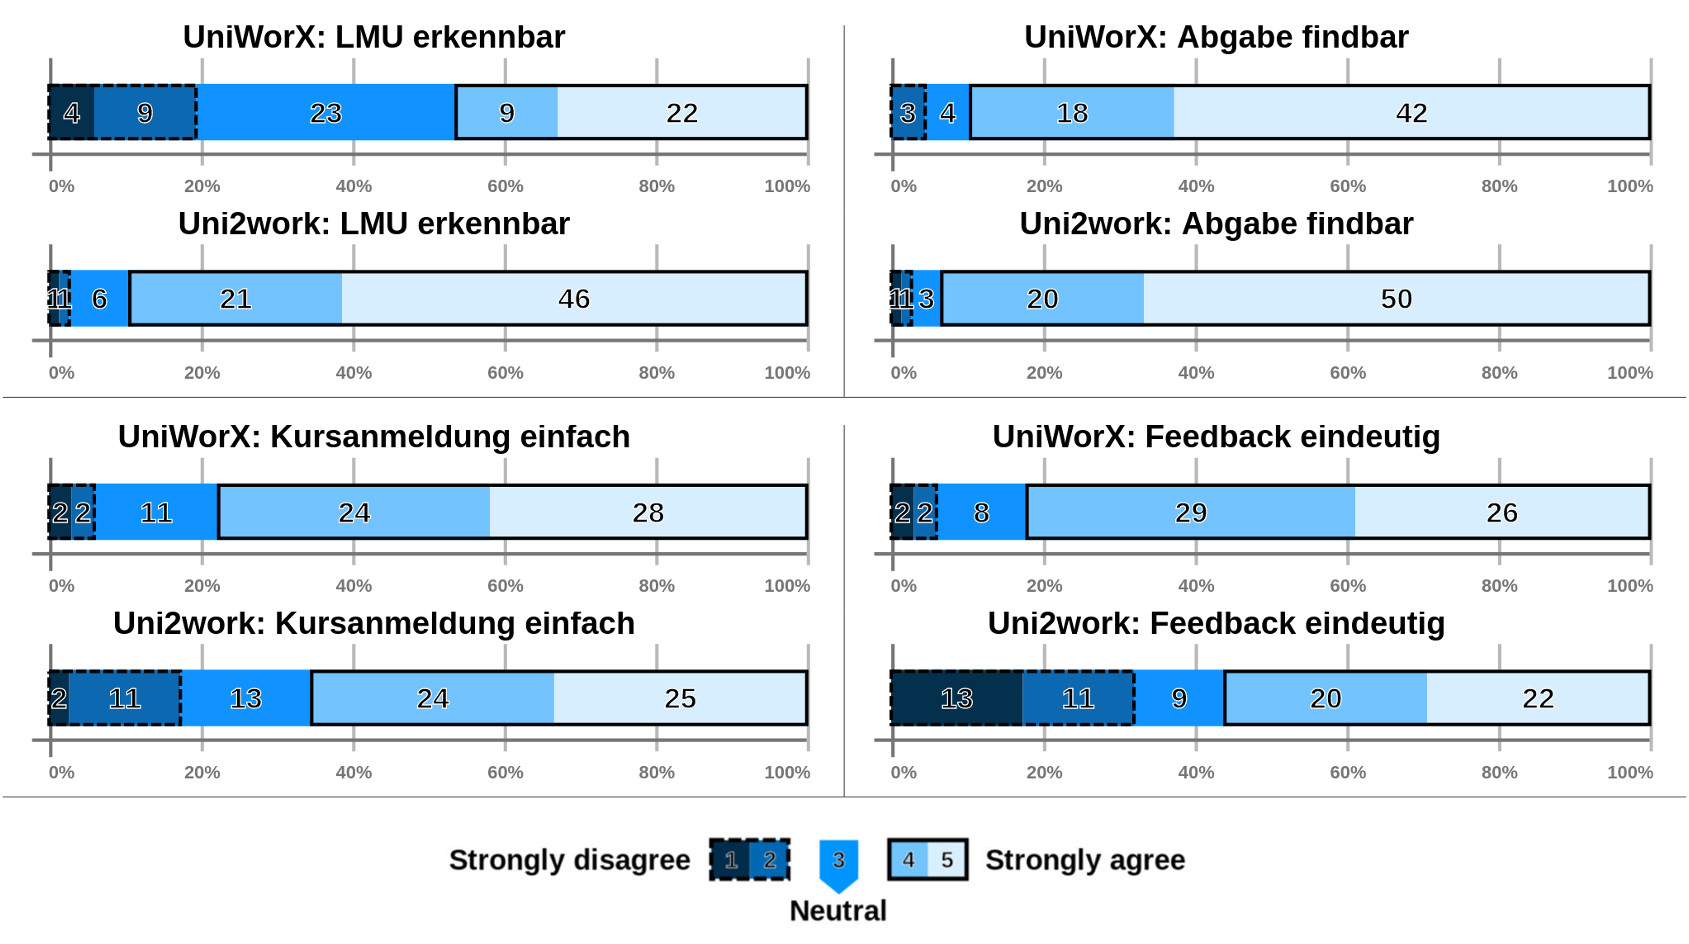
\includegraphics[width=\textwidth]{images/spezifragen.jpg}
    \caption{Gegenüberstellung der Reaktionen auf die Likert-Typ-Aussagen aus Sektion 5 des Fragebogens}
    \label{fig:system-specific-likerts}
\end{figure}

\subsection{Qualitative Analyse} \label{sec:results_qualitative}
In Sektionen 6 und 7 der Studie (siehe \autoref{sec:study_structure}) wurden die Teilnehmer gebeten Ihre Meinungen zu verschiedenen Aspekten in freier Textform niederzuschreiben. 
Unter den Antworten finden sich sowohl einfache Aussagen darüber was den Studenten an den Systemen besonders gut beziehungsweise besonders schlecht gefallen hat, als auch grundlegende und konstruktive Kritik.
Die freien Antworten der Teilnehmer wurden pro Frage in die Themen \textit{User Interface} und \textit{User eXperience} sortiert und werden hier vorgestellt:

\subsubsection{Was hat Ihnen besonders gut gefallen?}
\subsubsection*{UniWorX}
\hspace{6mm}\textbf{User Interface}
\begin{itemize}
    \item Verfügbarkeit von Farbthemen zur Personalisierung
\end{itemize}

\noindent\hspace{6mm}\textbf{User eXperience}
\begin{itemize}
    \item Übersichtliche und durchdachte Struktur
    \item Email-Benachrichtigungen und ihre fein gegliederte Anpassbarkeit
    \item Möglichkeit Feedback für Bewertungen zu hinterlassen
\end{itemize}

\subsubsection*{Uni2work}
\hspace{6mm}\textbf{User Interface}
\begin{itemize}
    \item Frisches, modernes Design
    \item Verfügbarkeit von Farbthemen zur Personalisierung
\end{itemize}
    
\noindent\hspace{6mm}\textbf{User eXperience}
\begin{itemize}
    \item Übersichtliche und durchdachte Struktur
    \item Sinnvolle Aufteilung der Navigation
    \item Gute Performanz / Schnelles Laden der Seiten
    \item Praktische Untermenüs die sich durch Hovern \footnote{Das Verweilen mit dem Mauszeiger über einem Webseiten-Element} öffnen
\end{itemize}

\noindent
Sowohl UniWorX als auch Uni2work wurden für ihre übersichtliche und durchdachte Struktur gelobt. Auch die Verfügbarkeit verschiedener Farbthemen aus denen die Benutzer wählen können und das System somit etwas personalisieren können wird begrüßt.
Als wichtiger Punkt auf UniWorX-Seite sind hier die Email-Benachrichtigungen anzusehen, welche für Uni2work zwar fest eingeplant sind, jedoch noch nicht vollständig implementiert wurden.

Aussagen wie "`An UniWorX hat man sich mittlerweile gewöhnt und es funktioniert gut"' verdeutlichen den positiven Einfluss der Bekanntheit des Systems auf die individuelle Bewertung. Zu Beginn als unpraktisch oder lästig empfundene Eigenschaften des Systems sind nach teilweise mehrjähriger Benutzung akzeptiert worden und werden nicht mehr negativ wahrgenommen. Mehr zu dieser menschlichen Eigenschaft in \autoref{sec:results_discussion}.

\subsubsection{Was hat Ihnen besonders schlecht gefallen?}
\subsubsection*{UniWorX}
\hspace{6mm}\textbf{User Interface}
\begin{itemize}
    \item Keine optische Verbindung zu anderen LMU-Seiten
\end{itemize}
    
\noindent\hspace{6mm}\textbf{User eXperience}
\begin{itemize}
    \item Unübersichtlichkeit der Veranstaltungs-Liste
    \item Keine Filter-Möglichkeit der Veranstaltungen
    \item Nur Informatik-nahe Veranstaltungen verfügbar
\end{itemize}

\subsubsection*{Uni2work}
\hspace{6mm}\textbf{User eXperience}
\begin{itemize}
    \item Schlechte Übersicht über bereits abgegebene Übungsblätter
\end{itemize}

\noindent
Ein großer Kritikpunkt an UniWorX welcher maßgeblich zu der Entwicklung des neuen Systems beigetragen hat war die Verfügbarkeit von ausschließlich Informatik-nahen Veranstaltungen im System. Einige wenige Veranstaltungen des Mathematik-Instituts wurden in den vorangegangenen zwei Semestern dem Veranstaltungs-Katalog von UniWorX hinzugefügt, der Großteil der übrigen Veranstaltungen anderer Institute und Fakultäten jedoch nicht.
Bereits in der Umfrage die zum Ende der Beta-Phase von UniWorX 2 durchgeführt wurde (s. \autoref{sec:uniworx_survey}) äußerten die Befragten den Wunsch alle Veranstaltungs-Anmeldungen zentral an einem Ort verwalten zu können. Die Auswertung dieser aktuellen Umfrageergebnisse hat gezeigt, dass dieser Wunsch fortbesteht. Auf die Umsetzung und die generelle Realisierbarkeit dieses Wunsches wird in \autoref{sec:future_work} eingegangen.

\subsubsection{Was würden Sie verbessern?}
\subsubsection*{UniWorX}
\hspace{6mm}\textbf{User Interface}
\begin{itemize}
    \item Verwendbarkeit auf kleinen Bildschirmen
\end{itemize}
    
\noindent\hspace{6mm}\textbf{User eXperience}
\begin{itemize}
    \item Bessere Performanz - vor allem bei Seiten mit langen Listen
    \item Verfügbarkeit der Materialien eines Kurses über UniWorX
    \item Filter- und Suchfunktion für Veranstaltungen (nach Abschluss, Studiengang, Fakultät, Prüfungsordnung, etc.)
    \item Automatisch generierter Stundenplan
\end{itemize}

\subsubsection*{Uni2work}
\hspace{6mm}\textbf{User Interface}
\begin{itemize}
    \item Übersichtlichere Kurs-Seiten
    \item Farbliche Hinweise auf die Dringlichkeit einer Abgabe (rot wenn <24h)
\end{itemize}
    
\noindent\hspace{6mm}\textbf{User eXperience}
\begin{itemize}
    \item Eindeutigere und besser erkennbare Statusmeldungen und Rückmeldungen des Systems
    \item Dedizierte Klausuren-Seite als neues Element der Hauptnavigation
    \item Drag \& Drop für Dateiuploads
\end{itemize}

\noindent
Der mehrfach geäußerte Wunsch der verbesserten Bedienbarkeit auf kleinen Bildschirmen wurde bei der Umsetzung des neuen Systems Uni2work von vornherein berücksichtigt.

Auch die Ladezeiten wurden reduziert. In UniWorX wurden Seiten mit verhältnismäßig langen Listen (über 200 Einträge) als langsam beschrieben. 
Auf Seiten ohne lange Listen, wie der Kursseite für "`Programmierung und Modellierung"' (s. \autoref{fig:uni2work_promo}) konnte die Ladezeit bis zum \textit{First Meaningful Paint} \footnote{Zeitpunkt beim Ladevorgang einer Webseite ab welchem der Betrachter das Endresultat der Seite erahnen kann} um knapp 40\% reduziert werden.
\textit{Lighthouse Audits} (Performanz-Messung) des Browsers \textit{Google Chrome} zeigen, dass UniWorX bereits sehr gute Ergebnisse erzielt, diese aber bei Uni2work noch deutlich verbessert werden konnten. Die Messungen, deren Ergebnisse in \autoref{fig:uniworx_lighthouse} und \autoref{fig:uni2work_lighthouse} zu sehen sind, wurden mit identischen Einstellungen vorgenommen. Beide Systeme erreichen, bei gleicher Konfiguration \footnote{Kein Network-Throttling (30MBit/s Downstream), kein Device-Throttling, Messung nach einem Neuladen der Seite}, ein Endresultat von 100 aus 100 Punkten, wobei bei Uni2work zusätzlich manche Zeiten um mehr als die Hälfte reduziert wurden im Vergleich zu UniWorX.

Weil in Uni2work bisher noch keine Seiten mit derart langen Listen existieren, konnte deren Ladezeit dort nicht gemessen werden und ein Vergleich mit UniWorX ist nicht möglich. Die Evaluierung der Ladezeiten auf solchen Seiten könnte Bestandteil einer Folgestudie werden. Die bisher nachvollziehbare Ladezeitenoptimierung ist jedoch bereits ein guter Indikator für die Geschwindigkeit des Systems.

Der Wunsch die Materialien einer Veranstaltung direkt über die Oberfläche von UniWorX herunterladen bzw. zumindest einsehen zu können, wurde bereits in der Umfrage zu UniWorX 2 erkannt. Dieser Wunsch wird unter anderem in \autoref{sec:future_work} diskutiert.

Die Möglichkeit der Filterung und eine Kategorisierung der Veranstaltungen wurde bei der Umsetzung von Uni2work bereits grundlegend berücksichtigt. Für eine voll funktionsfähige Suchfunktion und größeren Funktionsumfang der Filterfunktion bedarf es weiterer Arbeit, auf die in \autoref{sec:future_work} eingegangen wird.

\begin{figure}[h]
    \centering
    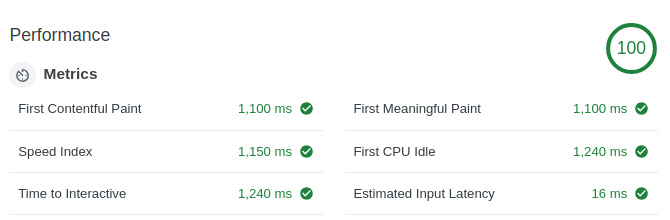
\includegraphics[width=.8\textwidth]{images/uniworxlighthouse.png}
    \caption{UniWorX: Performanz-Messdaten eines Lighthouse-Audit in Chrome. Das Resultat von 100 Punkten und die einzelnen Messwerte weisen bereits auf sehr geringe Ladezeiten hin. Für das Audit wurde kein Device- oder Netzwerk-Throttling aktiviert.}
    \label{fig:uniworx_lighthouse}
\end{figure}

\begin{figure}[h]
    \centering
    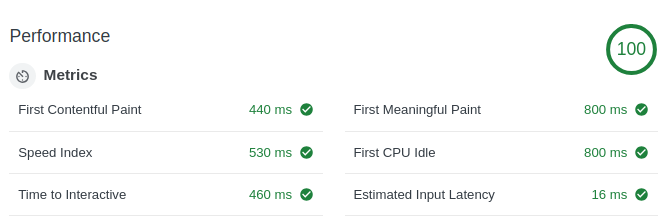
\includegraphics[width=.8\textwidth]{images/uni2worklighthous.png}
    \caption{Uni2work: Performanz-Messdaten eines Lighthouse-Audit in Chrome. Das Resultat von 100 ist wie bei UniWorX ein guter Indikator für hervorragende Performanz. Im Vergleich mit UniWorX konnten die einzelnen Messwerte zusätzlich teilweise um etwa die Hälfte reduziert werden. Für das Audit wurde kein Device- oder Netzwerk-Throttling aktiviert.}
    \label{fig:uni2work_lighthouse}
\end{figure}

\subsubsection{Usability von Uni2work auf kleinen Bildschirmen}
In Sektion 7 des Fragebogens (s. \autoref{sec:study_structure}) wurde nach der freien Meinung zur Usability von Uni2work auf Geräten mit kleinen Bildschirmen gefragt. Die Rückmeldungen auf diese sehr frei formulierte Frage waren überwiegend positiv. Gelobt wurde die Favoriten-Leiste die nur bei Bedarf eingeblendet wird (vgl. \autoref{fig:uni2work_mobile_favorites}) und die Menü-Leiste die dank aussagekräftiger Icons intuitiv zu verstehen und leicht zu bedienen ist. Kritisiert wurde mehrmals die Anzeige von Tabellen für die teilweise horizontal gescrolled werden muss um alle Spalten zu sehen. Sichtbar ist das etwa in dem Screenshot von Uni2work in \autoref{fig:mobile_comparison_uni2work}, in welcher die Tabelle der Abgaben auf der rechten Seite abgeschnitten ist. Bisher konnte keine zufriedenstellende alternative Darstellungsweise gefunden werden. Die Kritik wurde jedoch zur Kenntnis genommen und soll Bestandteil der weiteren Entwicklung von Uni2work sein, weswegen es in die in \autoref{sec:workflow} erwähnte Ticket-Liste aufgenommen wurde.

\subsection{Diskussion \& Auswertung} \label{sec:results_discussion}
Der berechnete SUS-Wert für das alte System liegt um knapp sechs Prozentpunkte über dem für das neue System. Obwohl dieser Unterschied keinen gravierenden Einschnitt in der Usability offenbart kam er für den Autor überraschend.

Zum Zeitpunkt der Durchführung der Studie befanden sich deutlich spürbare Bugs in Uni2work. Die unterschiedlichen Tabellen-Formatierungen welche in der Auswertung von Q5 in \autoref{sec:results_sus} bereits angesprochen wurden waren unter den deutlich spürbaren Inkonsistenzen des Systems. Eine weitere Lücke in der Funktionalität war ein irreführender \textit{Kurse}-Button in der Hauptnavigation, welcher -- mangels vollständiger Implementierung -- wider Erwarten auf eine Semester-Übersicht führte. Überdies stellte sich im Verlauf der Studie heraus, dass der essentielle \textit{Senden}-Button zum Hochladen erledigter Übungsaufgaben im Browser \textit{Safari} nicht funktionierte. Obgleich während der Studie an diversen Stellen des Systems auf den unvollständigen Zustand Uni2works hingewiesen wurde, dürften diese Eindrücke die Bewertung negativ beeinflusst haben.

Bangor et al. versuchten nach langjährigem Einsatz des SUS die resultierenden Werte auf eine Skala Menschen-verständlicher Adjektive zu übertragen \cite{bangor_sus_adjective}. Auf der in \autoref{fig:adjective_sus} gezeigten resultierenden Adjektiv-Skala von Bangor et al. bewegen sich beide Systeme im Bereich zwischen "`Gut"' und "`Exzellent"'.

Der Unterschied zwischen den SUS-Werten und insbesondere das schlechtere Abschneiden des neuen Systems kann zu einem gewissen Grad durch bekannte menschliche Phänomene und Effekte erklärt werden. Die Teilnehmer aus der UniWorX-Gruppe waren bereits vertraut mit dem System das sie bewerten sollten. Diese Tatsache hat potentiell die individuelle Bewertung leicht verfälscht. Menschen sind Opfer des \textit{Status-Quo Bias}, weshalb Sie bei einer Entscheidung zwischen \textit{Status-Quo} und \textit{Anders} überdurchschnittlich oft den aktuellen Zustand präferieren \cite{Samuelson1988}. Neben dem Status-Quo Bias existieren weitere Phänomene und Effekte die die Tendenz der Menschen beschreiben einem Verlust mehr Gewichtung zu verleihen als einem Gewinn \cite{endowmentkahnemann}. Da Änderungen immer mit dem Verlust des aktuellen Zustands einhergehen werden sie tendenziell eher vermieden oder zumindest mit Skepsis behandelt \cite{lewinresistance}.
Bereits die Tatsache, dass UniWorX als das "`alte System"' behandelt wird könnte seinen SUS-Wert positiv beeinflusst haben wie Eidelmann et al. 2010 gezeigt haben \cite{eidelmannlonger}.

Um die Hypothese der unterbewusst positiv beeinflussten Bewertung von UniWorX zu bestätigen bedarf es einer Folge-Studie nach einer angemessenen Zeit des Produktiv-Betriebs von Uni2work.

\begin{figure}[h]
    \centering
    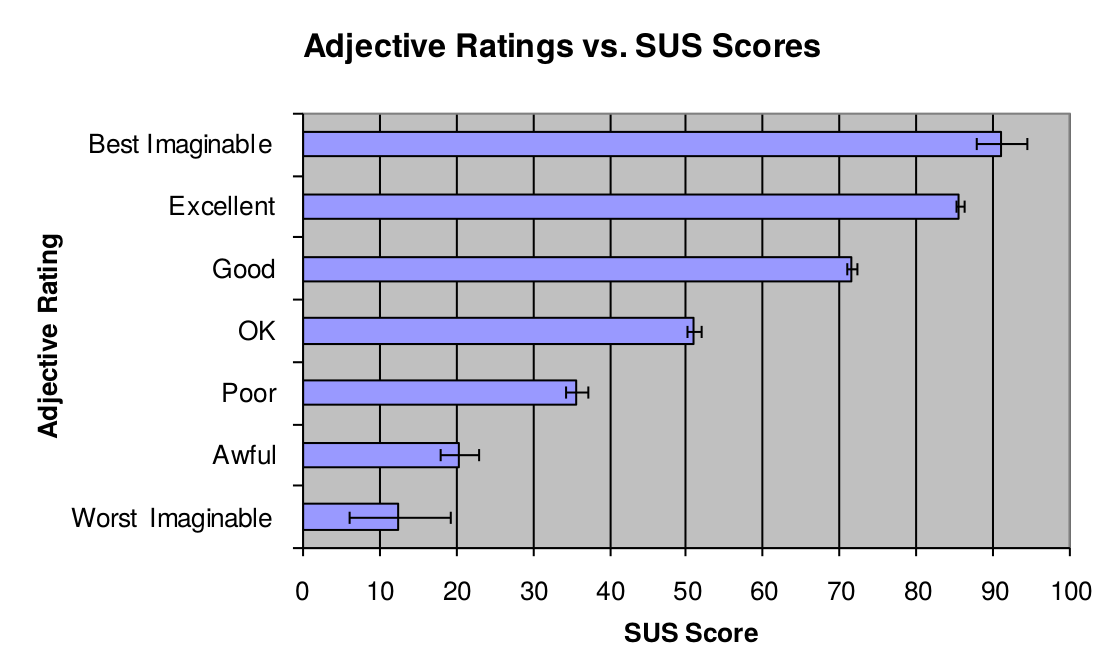
\includegraphics[width=\textwidth]{images/adjectivesus.png}
    \caption{Durschnittliche SUS-Werte und ihre entsprechenden Adjektive (mit Fehlerbalken für Standardunsicherheit) nach Bangor et al. \cite[S.119]{bangor_sus_adjective})}
    \label{fig:adjective_sus}
\end{figure}

\clearpage
\section{Rückblick \& Ausblick} \label{sec:future_work}
Die in \autoref{sec:userstudies} beschriebene Usability-Studie offenbarte keine Fehler im laufenden Betrieb. Diese Stabilität ist sicherlich dem Einsatz von Haskell zu verdanken. Die Implementierung von Uni2work ist jedoch weit davon entfernt als abgeschlossen bezeichnet zu werden. Neben den in \autoref{sec:results_discussion} angesprochenen Inkonsistenzen, welche seit dem Ende der Studie bereits großteils behoben wurden, gibt es nach wie vor Optimierungsbedarf. In den folgenden Unterabschnitten soll auf die, während der Implementierung gemachten Erfahrungen eingegangen werden und mit einem Überblick über zukünftige Arbeit abgeschlossen werden.

\subsection{Architektur}
Mit dem Einsatz von Haskell und dem verbundenen Kompilier-Vorgang ging eine gefühlte Sicherheit einher, die während der Entwicklung durchaus angenehm war. Bei geglückter Kompilierung liefen alle Funktionen fehlerfrei, der Vorgang selbst nahm jedoch jedes Mal eine vergleichsweise lange Zeit von letztendlich etwa 2 Minuten in Anspruch. Die Technologien die im Frontend eingesetzt werden können sind durch Haskell, bzw. den Einsatz von Yesod stark eingeschränkt oder mit erheblichem Aufwand verbunden. Während Yesod zwar den Einsatz von \textit{CoffeeScript} und \textit{TypeScript} \footnote{Alternativen zu nativem JavaScript die sich großer Beliebtheit erfreuen} statt Julius erlaubt, bestehen (laut offizieller Dokumentation) keine Alternativen zu Hamlet und Lucius/Cassius \cite{web:yesodstl}. Diese von Yesod zur Verfügung gestellten EDSLs (s. \autoref{sec:stl}) sind ausgereifte Sprachen die alles ermöglichen, das auch ihre Ziel-Sprachen HTML, CSS und JavaScript erlauben würden, bedurften jedoch einer gewissen Einarbeitung, gegeben den mangelhaften Haskell-Kenntnissen des Autors dieser Arbeit.

Der deutliche Unterschied zwischen den Backend- und Frontend-Technologien erschwerte die Kommunikation zwischen den Entwicklern vereinzelt. Änderungen die eine Seite der Entwicklung (Backend oder Frontend) als verhältnismäßig klein einstuften, stellten sich als nicht umsetzbar heraus oder waren nur mit großem Aufwand realisierbar. Ständigen Diskussionsstoff lieferte die Aufteilung der Hamlet-Bestandteile auf das Front- und das Backend.

Yesod bietet diverse Möglichkeiten zur Generierung von Hamlet-Snippets im Haskell-Quellcode, von denen auch bei der Implementierung von Uni2work Gebrauch gemacht wurde. Durch das Bereitstellen von vorgefertigtem Hamlet-Code direkt aus dem Backend fehlt dem Frontend an entsprechenden Stellen wichtiger Einfluss beispielsweise auf die Vergabe von Klassen für Style-Definitionen. Diese Snippets aus dem Backend werden per Widget-Interpolation (\lstinline!^{...}!, siehe \autoref{sec:interpolation}) in den Hamlet-Templates eingebunden, bieten aber keine weiteren Konfigurations-Möglichkeiten für Entwickler dieser Templates. Für die Umsetzung der sortierbaren Tabellenspalten, auf welche in \autoref{sec:einsatz-js} eingegangen wurde, war eine klar definierte HTML-Struktur von Nöten um JavaScript und CSS korrekt einsetzen zu können. Hierfür bedurfte es einiger Änderungen an der Art und Weise wie Yesod Tabellen für das Frontend produziert. TODO: finish this

\subsection{Zukünftige Arbeit}

- offene Tickets
- Barrierefreiheit. Accessibility-Tests (vielleicht Lighthouse Audits vergleichen?)
- deaktiviertes JavaScript -> Fehler
- Anmelde-Button auf Übersichts-Seite
- Alle Veranstaltungen in Uni2work
- Veranstaltungs-Webseiten in Uni2work
- Suche & Filter
- 

Ein Fehler der bereits vor der Durchführung der Studie gemeldet und repariert wurde war ein Problem mit den \textit{Senden}-Buttons unter Formularen. Ein Stück JavaScript (\textit{Julius}, s. \autoref{sec:stl}) das dafür sorgt, dass dieser Senden-Button deaktiviert wird und bleibt bis das Formular gültig ausgefüllt wurde hat in manchen Browsern (wie Safari) den Button nicht wieder korrekt aktiviert.

...

Mehrere Studenten haben angemerkt, dass Tabellen die breiter als der Bildschirm sind zwar mit horizontalem Scrollen betrachtet werden können, sich jedoch womöglich eine andere Form der Darstellung finden ließe mit der kein Scrollen notwendig wäre. Konkrete Ideen dazu wie eine solche Darstellung aussehen könnte waren in den Antworten nicht enthalten, wird aber definitiv bei der nächsten Ideenfindungs-Phase berücksichtigt werden.

%\_____________________________________________________________________

\clearpage
\section{Zusammenfassung} \label{sec:summary}
2nd (3rd) version of uniworx, evaluation outcome, 
4 to 5 sentences

\clearpage
\fancyhead[LE,RO,LO,RE]{} % Keine Kopfzeile mehr oben auf jeder Seite
\section*{Inhalt der beigelegten CD}

%______________________________________________________________________

\clearpage
\bibliographystyle{unsrt}
\bibliography{literature,webreferences}

\end{document}
